% AER-Article.tex for AEA last revised 22 June 2011
\documentclass[AER]{AEA}

%%%%%% NOTE FROM OVERLEAF: The mathtime package is no longer publicly available nor distributed. We recommend using a different font package e.g. mathptmx if you'd like to use a Times font.
\usepackage{mathptmx}

% The mathtime package uses a Times font instead of Computer Modern.
% Uncomment the line below if you wish to use the mathtime package:
%\usepackage[cmbold]{mathtime}
% Note that miktex, by default, configures the mathtime package to use commercial fonts
% which you may not have. If you would like to use mathtime but you are seeing error
% messages about missing fonts (mtex.pfb, mtsy.pfb, or rmtmi.pfb) then please see
% the technical support document at http://www.aeaweb.org/templates/technical_support.pdf
% for instructions on fixing this problem.

% Note: you may use either harvard or natbib (but not both) to provide a wider
% variety of citation commands than latex supports natively. See below.

% Margins
\usepackage[left=2.54cm,right=2.54cm,top=2.54cm,bottom=2.54cm]{geometry}
\usepackage{graphicx}
\usepackage{hyperref}

% Uncomment the next line to use the natbib package with bibtex 
\usepackage[spanish]{babel}
\usepackage[natbibapa]{apacite}
\bibliographystyle{apacite}
\usepackage[left=2cm,right=2cm,top=2cm,bottom=2cm]{geometry}
\bibliographystyle{aea}

% Uncomment the next line to use the harvard package with bibtex
%\usepackage[abbr]{harvard}

% This command determines the leading (vertical space between lines) in draft mode
% with 1.5 corresponding to "double" spacing.
\draftSpacing{1.5}
\setlength{\parindent}{2em}
\setlength{\parskip}{1em}
\renewcommand{\baselinestretch}{1.6}

\begin{document}

\title{Transferencias condicionadas en Colombia: ¿Cómo la asignación por puntaje del Sisbén a Familias en Acción afecta la accesibilidad a la educación?\footnote{El lector interesado podrá reproducir la totalidad del artículo utilizando las bases de datos y scripts realizados en R en el siguiente enlace: https://github.com/gecrodriguezpe/proyecto\_metodologia\_2.git}}
\shortTitle{Rodríguez, López y Pérez: Impacto del puntaje del Sisbén en el acceso a la educación}
\author{Germán Rodríguez, Juliana López and Raúl Pérez\thanks{Rodríguez: Universidad Nacional de Colombia (email gecrodriguezpe@unal.edu.co); López: Universidad Nacional de Colombia (email jvlopezne@unal.edu.co); Pérez: Universidad Nacional de Colombia (email rhperezp@unal.edu.co).}}
\date{\today}
\pubMonth{December}
\pubYear{2020}
\pubVolume{1}
\pubIssue{1}
\JEL{I21, I38, O12}
\Keywords{educación, transferencias monetarias condicionadas, evaluación de impacto, familias en acción}

\begin{abstract}
Se busca identificar cuál es el impacto que tiene la regla institucional de un puntaje de Sisbén por debajo de $30.56$ como mecanismo de asignación al programa Familias en Acción en el acceso a la educación por parte de los niños y jóvenes entre los 6 y 17 años de edad. Para realizar la identificación del impacto causal se usa un diseño de investigación basado en la ecuación asociada a la forma reducida de un Fuzzy RDD, dónde se usa como instrumento el puntaje de asignación al programa basado en el Sisbén. Todas las estimaciones se realizaron utilizando las bases de datos del Sisbén III proporcionadas por el DNP. Se encontró que efectivamente la regla institucional de asignación a familias en acción mediante el puntaje del Sisbén si tiene un efecto causal sobre la accesisibilidad a la educación para las personas en el rango de edad mencionando aumentando el acceso a la educación en un 5 \% en relación a la media para el rango de edad completo y en un 7 \% en relación a la media cuando se realizó la estimación de manera desagregada para los niños entre 6 a 11 años. Para los adolescentes entre 12 a 17 años no se encontró impacto significativo a la hora de hacer la estimación con este grupo de manera desagregada. 
\end{abstract}

\maketitle

% Raul y Juliana
\section{Introducción}
    
Tal como afirma \cite{deWalque2017CashDevelopment}, la pobreza tiene efectos significativos, perjudiciales y de largo alcance  en  el  desarrollo  infantil.   Es  por  esto que  a  lo  largo  de  la  historia  se  han  creado  programas  de \textit{transferencias de efectivo} con el fin de apoyar el desarrollo infantil y adolescente. En su desarrollo histórico los programas pioneros de Transferencias Monetarias Condicionadas (\textit{TMC}) empezaron principalmente en México y en Brasil en el año 1997 y posteriormente dichos programas de \textit{TMC} se han extendido a otros países de América Latina y, recientemente, a otros países en vías de desarrollo de otras regiones.
    
Según \cite{Sugiyama2011TheAmericas} el fundamento económico de los programas de \textit{transferencias condicionadas (CT)} es que pueden ser una forma equitativa y eficiente de abordar las fallas del mercado y llegar a las poblaciones más vulnerables \citep{Fiszbein2009ConditionalReport}. Así bien, como se sabe en la literatura, los programas de transferencias monetarias condicionadas están enfocados principalmente a que los estudiantes cumplan un requisito mínimo de asistencia a un programa escolar. No  obstante,  existen  otros  programas  de  transferencias  monetarias  condicionadas mucho  más amplios, que no solo tiene como exigencia asistir regularmente a un programa educativo si no también a cumplir cierta asistencia en chequeos de salud, entre otros.
     
En Colombia, el Programa Familias en Acción (FA) se diseñó y puso en marcha como una respuesta a los efectos de la crisis económica de finales de los años 1990, con el propósito de proteger y promover la formación de capital humano en las familias en extrema pobreza, a través del otorgamiento de subsidios condicionados a la asistencia escolar y al desarrollo de acciones de cuidado de la salud y la nutrición en poblaciones menores de 18 años \citep{Robles2018Las2001-2018}. 

Para ver la efectividad del programa se decidió identificar el impacto de éste en el acceso a la educación para los niños y jóvenes entre los 6 y 17 años. Utilizando las bases de datos del Sisbén III, facilitada por la Departamento Nacional de Planeación (DNP), que consistían en una muestra tipo panel con información de inscritos en el Sisbén entre el año 2011 y 2016, se identifico el impacto que tiene la regla institucional de un puntaje de Sisbén por debajo de $30.56$ como mecanismo de asignación al programa Familias en Acción en el acceso a la educación por parte e los niños y jóvenes entre los 6 y 17 años de edad. La razón para no medir directamente el impacto del programa familias en acción en el acceso a la educación y en lugar usar el puntaje de asignación al programa vía puntaje del Sisbén se debe a razones metodológicas relacionadas con la base de datos empleada como se mencionará más adelante en más detalle. 

Para realizar la identificación del impacto causal se usa un diseño de investigación basado en la ecuación asociada a la forma reducida de un Fuzzy RDD, dónde se usa como instrumento el puntaje de asignación al programa basado en el Sisbén. Se encontró que efectivamente la regla institucional de asignación a familias en acción mediante el puntaje del Sisbén si tiene un efecto causal sobre la accesisibilidad a la educación para las personas en el rango de edad mencionando aumentando el acceso a la educación en un 5 \% en relación a la media para el rango de edad completo y en un 7 \% en relación a la media cuando se realizó la estimación de manera desagregada para los niños entre 6 a 11 años. Para los adolescentes entre 12 a 17 años no se encontró impacto significativo a la hora de hacer la estimación con este grupo de manera desagregada. 

Se destaca que el impacto causal identificado confirma y refuerza los resultados obtenidos en la literatura y en otros trabajos empíricos de que los programas de transferencias monetarais condicionadas han sido políticas públicas efectivas en incentivar la asistencias escolar en los países latinoaméricanos y otros países en vías de desarrollo. La magnitud del impacto identificado, también da una sugerencia de posibles formas de aumentar la efectividad del programa como lo son complementarlo con programas que subsidien la oferta o buscando otros mecanismos de focalización distintos al sisbén. 

El artículo procede de la siguiente forma. La sección I es la introducción. La Sección II provee un Estado del arte de como se ha abordado las TMCs en general y el programa de familias en acción en particular. La sección III mira la justificación de la intervención de Familias en acción y el contexto detrás de él en Colombia. La Sección IV presenta los datos utilizados y las modificaciones necesarias para poder realizar las estimaciones. La Sección V presente el diseño de investigación empleado para realizar las estimaciones mientras que la sección VI muestra los principales resultados al emplear el diseño de investigación en la base de datos utilizada. Finalmente, la sección VII concluye. 

\section{Estado del arte}

En su desarrollo histórico los programas pioneros de TMC empezaron principalmente en México y en Brasil en el año 1997, posteriormente las TMC se han extendido a países de América Latina y más allá, según \cite{Sugiyama2011TheAmericas}. El programa pionero Progresa en México empezó con aproximadamente 30.000 familias y hoy cubre a 5 millones de familias. Según \cite{Schultz2004SchoolProgram} este es un programa que evalúa el impacto del programa en la matrícula de los niños más pobres de las zonas rurales de México. También muestra cómo este programa no solo tuvo efectos a corto plazo en esta población, sino el efecto positivo en la escolaridad de por vida del individuo. Para el año 2017, el programa federal Bolsa Família, programa heredero del programa Bolsa Escola que fue el otro programa pionero en TMC's, atiende a 11 millones de familias (46 millones de personas) \citep{Fiszbein2009ConditionalReport}. Ya en el 2008, virtualmente casi todos los países latinoamericanos tenían alguna especie de transferencia condicionada. En otras partes del mundo, Bangladesh, Indoneisa y Turquía se han caracterizado por tener programas de TMC's de gran escala, mientras que Cambodia, Malawi, Marocco, Pakistan y Sudafrica para ese mismo año adoptaron programas pilotos sobre TMS's \citep{Fiszbein2009ConditionalReport}.

\cite{Soares2007ConditionalPaper} dado que este fue uno de los primeros documentos que se preocupo por medir el impacto que puede tener las TMC en la reducción de la desigualdad. Estando en los resultados más destacados el pequeño impacto que tuvo en la reducción del índice GINI.\cite{Soares2010EvaluatingPerspective} indaga un poco más sobre el impacto del programa Bolsa Familia en donde concluye que el programa Bolsa Familia ha tenido un impacto positivo en la participación laboral adulta, con un impacto mayor sobre las mujeres.

Existen otros programas de transferencias monetarias condicionadas, mucho más amplios que tienen más condiciones. \cite{Lagarde2007ConditionalReview} analizando 6 programas distintos de TMCs llega a la conclusión que dichos programas son moderadamente efectivos en incrementar el uso de los servicios de salud y mejorar resultados nutricionales sobre la población tratada así como incentivar comportamientos preventivos de salud. 

Y a medida que los TMCs empezaron a captar el interés de muchos investigadores del desarrollo y de gobiernos de África subsahariana, \cite{Baird2011} mediante un RCT aplicado a comunidades rurales de Malawi, queriendo ver si era necesario que las transferencias monetarias fueran o no fueran condicionadas. El artículo concluyó que en el grupo tratamiento, que fue le que recibió las transferencias condicionadas, hubo un aumento sustancial en la asistencia a los colegios y además obtuvo mejores desempeños en las pruebas académicas en comparación al grupo control que solo recibió las transferencias monetarias condicionadas. 

No obstante, además de \cite{Baird2011} otros autores han intentando hacer aportes a la interrogante  de si las transferencias monetarias deberían ser condicionadas o no. Autores como \cite{DeBrauw2011MustMexico} realizando un estudio para México y \cite{NorbertSchady2008CashEcuador} para ecuador encontraron en experimentos parecidos a los realizados por \cite{Baird2011} que la asistencia escolar era significativamente inferior en las personas que hacían parte del grupo control frente a las que hacían parte del grupo tratamiento.

Se desarrollaron más artículo relacionados con el uso de RCTs para el estudio del impacto de las transferencias monetarias condicionadas en donde la mayoría de estudios tuvieron efecto en Africa subsahariana. Mediante un experimento controlado, \cite{Asfaw2014CashKenya} realizaron un RCT en Kenya cuyo objetivo era investigar el impacto de un programa de transferencias condicionadas para los programas para huérfanos y niños en condiciones de vulnerabilidad en las decisiones acerca de actividades productivas por parte de los hogares que adoptan a dichos niños.

Tres mecanismos de focalización para la selección de hogares en dichos programas se conocen como Proxy Means Testing (PMT),en el cual se usan los activos para definir que hogares tratar, Community-Based Targeting (CBT), donde la misma comunidad hace un ranking de cuales son los hogares más pobres, y un método híbrido que combina a los dos. En la literatura hay consenso de que el mecanismo PMT es más efectivo que los mecanismos que emplean CBT como lo encontraron \cite{Alatas2012TargetingIndonesia} en su estudio experimental para Indonesia y como lo confirma \cite{Stoeffler2016ReachingCameroon} en una evaluación de un programa piloto de transferencias monetarias condicionadas, donde concluyes que hay que tener cuidado en utilizar los mecanismos de CBT dado que éstos son menos efectivos que PMT en la selección de hogares que requieran el programa y además que los CBTs pueden mejorar sustancialmente si se les realiza un seguimiento más regular, así como una mayor integración en el uso de los CBT junto a los PMT. 

Pero, para informar un poco más acerca de los impactos sobre los niños de los programas de transferencias monetarias condicionadas, se recurrió en primera instancia al trabajo de \citep{Ozer2009EffectsProblems}, \citep{Baird2010TheWomen} y \citep{Pettifor2012CanPrevention}. Dado que \cite{Ozer2009EffectsProblems} concluyen que este tipo de intervenciones estatales que se centran en invertir en las necesidades básicas de capital humano pueden ejercer un efecto dominó a más largo plazo en el desarrollo de los niños. Por otra parte, el trabajo de \cite{Baird2010TheWomen} afirman que los programas de transferencias condicionadas son efectivos para aumentar la matrícula y la asistencia escolar, sin embargo señalan que estos efectos ayudaron a su vez a la disminución de embarazos adolescentes pues ayudaba a evitar la actividad sexual. \cite{Pettifor2012CanPrevention} apoyan esta postura con su trabajo pues afirman que las transferencias monetarias condicionadas han tenido un impacto poco conocido en cuanto a  la prevención del VIH, realizando un estudio de los adolescentes de los países en desarrollo donde han sido implementadas estas intervenciones.

Pero, el alcance de los TMC, toca muchas más áreas. \cite{Kilburn2020The068} utilizando datos primarios estudiaron la intervención de transferencia de efectivo condicionada y aleatorizada para niñas en Sudáfrica que se desarrolló entre 2011 y 2015, mostrando que la transferencia de efectivo reduce consistentemente las diferentes formas de abuso que pueden afectar  a las niñas, en particular a través de los dominios de agencia económica, violencia y relaciones. \cite{Kennedy2014ExploringTanzania} Estudiaron la correlación entre el riesgo de contagiarse VIH con la pobreza y la desigualdad de género; Buscando explorar la viabilidad y la eficacia de una intervención de transferencia de efectivo para mujeres jóvenes en Iringa, Tanzania, demostrando que un programa de transferencia de efectivo ayudaba a reducir la instancia del VIH, las infecciones de transmisión sexual y los embarazos no deseados. 
 
Otros campos en los cuales los TMC pueden afectar las características socio económicas es presentado por \cite{Case2005HeKwaZulu-Natal} pues ellos examinaron el alcance e impacto de la subvención de manutención infantil de Sudáfrica, encontrando que los niños beneficiados tenían más probabilidades de matricularse en la escuela en los años posteriores a la recepción de la subvención que los otros niños. Concluyendo que a una mayor pobreza en los hogares que reciben subvenciones. Se permite evidenciar que el desarrollo infantil es sensible a los entornos de la vida temprana, y que los niños y niñas pobres tienen una probabilidad mayor de déficit cognitivos y conductuales, examinado por \cite{Paxson2010DoesAnd} al estudiar un programa de TMC administrada por el gobierno para madres pobres de Ecuador, el cual influyó en el desarrollo de los niños pequeños.

Ahora bien, enfocando el trabajo en Colombia \cite{Barrera-Osorio2007TheQuasi-experiment} evaluaron el impacto de un programa de reducción de tarifas lanzado por la ciudad de Bogotá en 2004. Encontraron que las reducciones de tarifas ofrecidas a las personas de los niveles 1 y 2 de Sisben tienen un efecto positivo en la inscripción en los grados primarios de los estudiantes de Sisben 1 y en los grados de secundaria para el Sisben 2. Específicamente, las estimaciones sugieren que Gratuidad aumenta la probabilidad de la matriculación para los estudiantes de Sisben 1 de edad primaria en aproximadamente un 3 por ciento, y para los estudiantes de Sisben 2 de secundaria en aproximadamente un 6 por ciento.

Las evaluaciones de impacto también demuestran que en las zonas rurales el programa aumenta el ahorro formal, la adquisición de bienes durables (como neveras), la probabilidad de acceder a crédito formal y desincentiva el ahorro informal \cite{Robles2018Las2001-2018}. Por lo anterior, dichos autores llegan a la conclusión de que en términos generales el programa tiene un impacto más notorio en las zonas rurales que en las urbanas.

 \cite{Robles2018Las2001-2018} menciona en su texto que Familias en Acción se ha convertido en uno de los programas sociales más evaluados en la historia reciente de Colombia y también uno de los cuáles más gasto público ha recibido como los autores muestran en su gráfico 7 de su investigación. Además, el programa ha logrado beneficiar miles de familias anualmente, desde 2001 hasta el 2017 \citep{Robles2018Las2001-2018}. Uno de los retos del programa familias en acción como lo muestran \cite{Robles2018Las2001-2018} es que hay que incentivar la oferta de los servicios ofrecidos por el programa, es decir cobertura en salud como en educación, tanto como la demanda para que el programa sea efectivo.

\cite{PulidoBuitrago2013LosAccion} con el propósito de recelar los efectos políticos y sociales que ha generado el programa Familias en Acción en los beneficiarios y en su relación con el Estado, examinó el surgimiento y la consolidación de los programas de (TMC) en América Latina desde mediados de los noventa como principales estrategias de la ‘lucha contra la pobreza’.

\section{Intervención y contexto}

En la década de los 90, Colombia paso por una gran crisis económica que afecto el consumo de los hogares al afectar sus ingresos, lo cual trajo como consecuencia una menor asistencia de los niños y jóvenes a los centros escolares. A raíz de eso el gobierno nacional mediante el Departamento Nacional de Planeación (DNP) implementó una política para velar por la educación de la población joven, el cual hoy se conoce como Familias en Acción.

Familias en Acción es el programa de Prosperidad Social que entrega a todas aquellas familias que se encuentran en estado de pobreza y extrema pobreza con niños, niñas y adolescentes un incentivo económico condicionado que complementa sus ingresos para la formación de capital humano, la generación de movilidad social, el acceso a programas de educación media y superior, la contribución a la superación de la pobreza y pobreza extrema y a la prevención del embarazo en la adolescencia. 

Además, se entrega un incentivo de salud y uno de educación, el de salud se entrega cada dos meses (6 veces al año) hasta el día antes que el niño o niña cumpla los 6 años, siempre y cuando asistan oportunamente a las citas de valoración integral en salud para la primera infancia en la respectiva Instituto Prestador de Salud (IPS). Y el incentivo de educación se entrega cada dos meses, menos en el período de vacaciones de fin de año escolar, es decir, cinco veces al año, siempre y cuando la familia cumpla con dos compromisos: los niños, niñas y adolescentes deben asistir como mínimo al 80\% de las clases programadas y no pueden perder más de dos años escolares. En el caso que uno de los participantes tenga 18 o 19 años debe estar cursando mínimo 10° grado, y si tiene 20 años grado 11°.


% Raul y Juliana
\section{Datos}

% Describir de donde provienen los datos 

Los datos para este análisis provienen de las bases de datos anonimizadas para el \textit{Sisbén III} para el corte de diciembre del 2016\footnote{Dicha base de datos se obtuvo por una solicitud directa que se realizó al Departamento Nacional de Planeación (DNP)}. Dado que hay varias bases de datos asociadas al Sisbén III para el corte de diciembre de 2016 las estimaciones se realizaron usando exclusivamente la base de datos llamada \textit{Sisben\_III\_PERS\_DIC2016.dta}. La última base de datos mencionada, se caracteriza por ser un panel que va del año 2011 al año 2016 en donde cada observación corresponde a una persona beneficiaria el Sisbén III en un determinado año. Es importante destacar que esta base de datos sufre dos importantes limitaciones: 1) No se tiene información sobre el año al que pertenece cada observación \textit{Por lo que se limita en gran medida los diseños de investigación que se pueden realizar con dicha base de datos} y 2) más importante para el presente estudio, es la carencia de una dummy que indique que observación es beneficiaria de familias en acción y que observación no lo es\footnote{Para más información sobre la base de datos empleada consultar: https://anda.dnp.gov.co/index.php/catalog/98}. 

Ahora bien, por la manera en la que fueron codificadas las variables desde el DNP fue necesaria realizar un tratamiento a la base de datos para adecuarla a las necesidades del estudio. Por tanto, las variables \textit{asistente a centro educativo}, \textit{sexo}, \textit{embarazada}, \textit{percibe ingresos} y \textit{estudio el último mes} debieron ser codificadas como variables dummys con valores discretos 0 y 1. De igual forma, la variable \textit{estudio el último mes} se definió con el valor de 1 si la persona había estudiado en el último mes y 0 si se había dedicado principalmente a realizar otra actividad distinta a estudiar. Finalmente, se filtró la base de datos de tal forma que se seleccionó solo dos grupos poblaciones: g1) consistía esencialmente de niños entre los a 6 a 11 años mientras que g2) consistía de adolescentes entre los 12 a los 17 años\footnote{La base de datos filtrada contenía un total de $22286$ observaciones.}. Lo último se debe a que se busca ver el efecto del \textit{programa familias en acción} en el acceso a la educación por lo que tiene sentido estudiar a las personas que hagan parte de estos grupos poblacionales.\footnote{En realidad el impacto que se identificó no fue el de familias en acción sobre el acceso a la educación sino el efecto que genera el umbral de $30.56$ para el puntaje de sisbén 3 en separar las potenciales familias beneficiarias del programa familias en acción de las familias que no pueden acceder al programa por superar este umbral en el acceso a la educación. Lo anterior se debe, principalmente, a limitaciones en la base de datos empleada como se explicará con mayor detalle en la sección de metodología}. 

Finalmente, la tabla \ref{tab:info_var}\footnote{Se resalta que si bien se menciona la variable tratamiento: \textit{Hace parte de familia en acción}, se resalta que dicha variable no se trabajará directamente ni se trabajará cuantitativemente sino que sirve como variable de referencia para el fuzzy RDD que se empleará como metodología empírica y de estimación.} muestra que variables se usaron en las estimaciones y qué miden así como su media muestral. 



\begin{table}[h]
\centering
\caption{Información variables claves}
\begin{tabular}{llll}
\hline
\hline
\textbf{Nombre de la variable}                                                                                                                                                                                                       & \textbf{Abreviación} & \textbf{Tipo de variable} & \textbf{Media} \\ \hline
\textbf{Variable Outcome (Respuesta):}                                                                                                                                                                                               &                      &                           &                \\
Estudio el último mes                                                                                                                                                                                                                   & EUM                  & dummy                     & 0.77           \\
\textbf{Variable tratamiento:}                                                                                                                                                                                                       &                      &                           &                \\
Hacer parte de familias en acción                                                                                                                                                                                                     & FeA                  & dummy                     & NA             \\
\textbf{Instrumento:}                                                                                                                                                                                                                &                      &                           &                \\
\begin{tabular}[c]{@{}l@{}}Umbral del sisbén que separá potenciales \\ beneficiaris de familias en acción de\\  persona que no pueden acceder \\ el programa por exceder el valor crítico\\ $T_i = 1(PS3_i \geq 30.56)$\end{tabular} & T                    & dummy                     & 0.25           \\
\textbf{Covariadas:}                                                                                                                                                                                                                 &                      &                           &                \\
Sexo                                                                                                                                                                                                                                 & S                    & dummy                     & 0.52           \\
Embarzada                                                                                                                                                                                                                            & E                    & dummy                     & 0.26           \\
Pecibe ingresos                                                                                                                                                                                                                      & I                    & dummy                     & 0.072          \\
\textbf{Running variable:}                                                                                                                                                                                                           &                      &                           &                \\
Puntaje del Sisbén III                                                                                                                                                                                                               & PS3                  & variable continua         & 22.5      \\ \hline
\end{tabular}
\label{tab:info_var}
\end{table}


% Raul y Juliana
% german

\section{Metodología}

Dado que existe una regla institucional bien establecida que indica que las personas que cuentan con un puntaje de Sisbén por encima de $30.56$ están inhabilitadas a \textit{acceder al programa familias en acción} mientras que las personas con puntaje menor pueden ser posibles beneficiarios del programa se tiene que si uno se concentra alrededor del umbral que separa ambos grupos, es decir $30.56$, se tendría una especie de experimento natural alrededor de dicho umbral donde la asignación al tratamiento, en este caso pertenecer o no pertenecer a familias en acción, se puede ver como una asignación aleatorizada o una loteria alrededor del umbral. Este es el caso, porque algunas personas por poco superaron el umbral de asignación $30.56$ mientras que otras personas por poco no lo superaron sin que estas personas tengan control directo sobre dicha asignación\footnote{Sobre esta última afirmación relacionada con no manipulación por parte de los individuos se hablará un poco más en la sección de resultados.}

\subsection{Fuzzy RDD}

Por lo anterior, un diseño de investigación basado en un \textit{Regression Discontinuity Design (RDD)} sería propicio dado que dicho diseño se basa en estimar un efecto alrededor de un umbral establecido que separa al grupo tratado del no tratado \citep{Lee2010RegressionEconomics}\footnote{La definición dada acá es la asociada a un \textit{Sharp} RDD donde hay perfecto cumplimiento al tratamiento, es decir, si una persona es asignada al tratamiento dicha persona cumple con el rol que se le asigno}. No obstante, como lo expresan \cite{Lee2010RegressionEconomics} en caso tal de que no haya perfecto cumplimiento al tratamiento\footnote{Es decir, los individuos no cumplen perfectamente con el rol que se les dio en la asignación} o existan otras formas de asignación al tratamiento además de la regla institucional/umbral es necesario emplear lo que se conoce como un \textit{fuzzy RDD}\footnote{Se recuerda al lector que un fuzzy RDD consiste en 3 ecuaciones principales: 1) ecuación estructural, 2) una primera etapa y 3) una forma reducida siguiendo un enfoque idéntico al de un diseño de investigación por variable instrumental donde el umbral/regla institucional que determina la asignación al tratamiento actua virutualmente como instrumentod de la variable de asignación \citep{Cunningham2018CAUSAL1.7}. La diferencia entre un \textit{Sharp RDD} y un \textit{Fuzzy RDD} es excatamente paralela a la diferencia entre un RCT con perfecto cumplimiento y un RCT con incumplimiento en la asignación, dónde a intención a tratar es aletorizda \citep{Lee2010RegressionEconomics}. Es por ello que la estructura de un Fuzzy RDD sigue un diseño de investigación por varible instrumental}. En nuestro presente estudio, el uso del fuzzy RDD es necesario dado que que existen cuatro mecanismos diferentes por medio del cual se puede asignar familias en acción, uno de ellos es el puntaje del Sisbén (Regla institucional), mientras que los otros 3 son asignaciones a población desplazada, población indígena y personas que hagan parte Red Unidos   \citep{Robles2018Las2001-2018}. La presencia de otros mecanismos hace que algunas personas con un puntaje del sisbén de $30.56$ puedan acceder al programa a pesar de que por la regla institucional no debería. 
 
Siguiendo la metodología de \cite{Angrist2008MostlyCompanion} la ecuación estructural del fuzzy RDD para la investigación planteada está dada por la ecuación \ref{eq:estructural}.\footnote{Dicha ecuación corresponde a un diseño local lineal discontinuo que estima el impacto que tendría la asignación de familias en acción en el acceso a la educación para las personas que se encuentran cerca al umbral institucional.} 

\begin{equation}
    EUM_i = \alpha + \beta_1 PS3_i + \rho FeA_i + \eta_i
    \label{eq:estructural}
\end{equation}

Donde $FeA$ es la \textit{variable de asignación al tratamiento}, $PS3_i$ es la \textit{running variable} y $EUM_i$ es la \textit{variable outcome o resultado}. Ahora bien, la ecuación de la primera etapa del fuzzy RDD está dada por \ref{eq:fist_stage}.\footnote{Dicha ecuación estima el impacto que tiene el instrumento/intención a tratar $T_i$ sobre la variable de asignación $FeA_i$.}

\begin{equation}
    FeA_i = \gamma_0 +  \gamma_1 PS3_i + \pi T_i + \xi_{1i}
    \label{eq:fist_stage}
\end{equation}

Donde $T_i$ es el instrumento para la variable $FeA_i$\footnote{Cómo ya se mencionó, un fuzzy RDD se puede ver como un sharp RDD con incumplimiento perfecto por lo que la variable de asignación requiere un instrumento. En palabras de \cite{Angrist2008MostlyCompanion} un fuzzy RDD es un diseño de investigación donde el umbral donde ocurre la discontinuidad se convierte en una variable instrumental para el estado tratamiento. Dicho instrumento se puede ver como la intención a tratar, en este caso como los individuos que por regla institucional podrían o no acceder al programa familias en acción dado su puntaje del Sisbén.}. Finalmente, y como ya se manifestó en la sección de datos, la base de datos del Sisbén III con la que se hizo la estimación tiene la desventaja de no tener información de que personas en realidad accedieron a familias en acción y quienes no lo hicieron, y tan solo tiene explícitamente el puntaje del Sisbén, por lo que es necesario estimar la forma reducida del fuzzy RDD para poder estimar algún impacto causal. Si se reemplaza la ecuación \ref{eq:fist_stage} en \ref{eq:estructural} se obtiene la ecuación que da la forma reducida \ref{eq:reduced_form}.\footnote{Dicha ecuación estima el impacto directo que tiene el instrumento/intención a tratar $T_i$ sobre la variable outcome/resultado $EUM_i$.}

\begin{equation}
    EUM_i = \mu + \kappa_1 PS3_i + \rho \pi T_i + \xi_{2i}
    \label{eq:reduced_form}
\end{equation}

Dado que la ecuación \ref{eq:reduced_form} se puede estimar por medio de un \textit{diseño de regresión lineal local discontinuo} se tiene que el impacto causal de interés está dado por \ref{eq:impacto} \footnote{Éste es el parámetro causal de interés  que se planea identificar en este artículo por medio de  estimar directamente la forma reducida en lugar de estimar todo el fuzzy RDD (Dado que no se conoce la asignación a tratamiento $FeA$ por las limitaciones propias de la base de datos usada). De igual forma, mientras que en un fuzzy RDD el impacto que se termina estimando es un \textit{Local Average Treatmen Effect (LATE)} que debe satisfacer además de los supuestos usuales de un RDD la \textit{restricción de exclusión} y el \textit{supuesto de monotonicidad} para un \textit{diseño de investigación por variable instrumental} se tiene que al estimar solo la forma reducida \ref{eq:reduced_form} en el presente artículo ya no es necesario satisfacer el supuesto de monotonicidad ni la restricción de exclusión y que el impacto causal \ref{eq:impacto} si se puede interpretar como un \textit{Average Treatmente Effect (ATE)} para los individuos que se encuentran cerca al umbral de corte \citep{Imbens1994IdentificationEffects}}.

% agregar lo de que ese efecto se interpreta como un ATE distinto a un LATE que sería el caso de un fuzzy RDD y citar al otra Angrist e Irving

\begin{equation}
    \rho \pi = \lim \limits_{PS3 \to 30.56^{+}} E[EUM | PS3 = 30.56] - \lim \limits_{PS3 \to 30.56^{-}} E[EUM | PS3 = 30.56] \label{eq:impacto}
\end{equation}

% german
\section{Resultados}

\subsection{Estimación principal}

% Presentar los resultados de no manipulación

Dado los cuatro mecanismos existentes de asignación a familias en acción y dado que la base de datos no contiene explícitamente que personas son beneficiarias del programa y que personas no lo son, las estimaciones se centraran en estimar la forma reducida \ref{eq:reduced_form} donde el impacto que eventualmente se identificará será el impacto de la intención a tratar sobre el acceso a la educación dado por \ref{eq:impacto}. Dado que, en la ecuación para la forma reducida $T_i$ se puede interpretar como la intención a tratar o a dar familias en acción a partir del puntaje del sisbén\footnote{Nuevamente, se recuerda al lector que en este caso se asumirá que si tiene un puntaje por encima de 30.56 no será parte de familias en acción mientras que si tiene un puntaje mejor a 30.56 será beneficiario en familias en acción aunque en la práctica esto no es estrictamente cierto por incumplimiento perfecto (algunas personas que podrían ser beneficiadas simplemente deciden por motivos personales u otras razones hacer parte del programa) o por los otros tres mecanismos de asignación a familias en acción que existen.} la estimación de \ref{eq:reduced_form} se puede realizar mediante un \textit{Sharp RDD} donde es necesario que se cumpla los supuestos de: 1) no manipulación por parte de los individuos que se encuentran alrededor del umbral y 2) que la única variable que salta en el umbral es la intención a tratar $T_i$, es decir, que haya continuidad en las otras covariadas empleadas en el modelo\footnote{Dado que si alguna otra variable salta además de la intención a tratar entonces se puede tener otra explicación plausible alternativa.} \citep{Cunningham2018CAUSAL1.7}.\

La no manipulación por parte de los individuos alrededor del umbral está garantizada tanto por el contexto institucinal como por los resultados estadísticos. Del contexto institucional, a la hora de asignar el puntaje del Sisbén a cada individuo el DNP lo hace con una \textit{fórmula secreta o al menos desconocida} para los posibles beneficiarios y luego de que éstos son entrevistados por lo que es muy improbable que haya manipulación del puntaje de éstos alrededor del umbral de asignación a familias en acción por medio de dicho puntaje. 

\begin{figure}[h!]
    \centering
    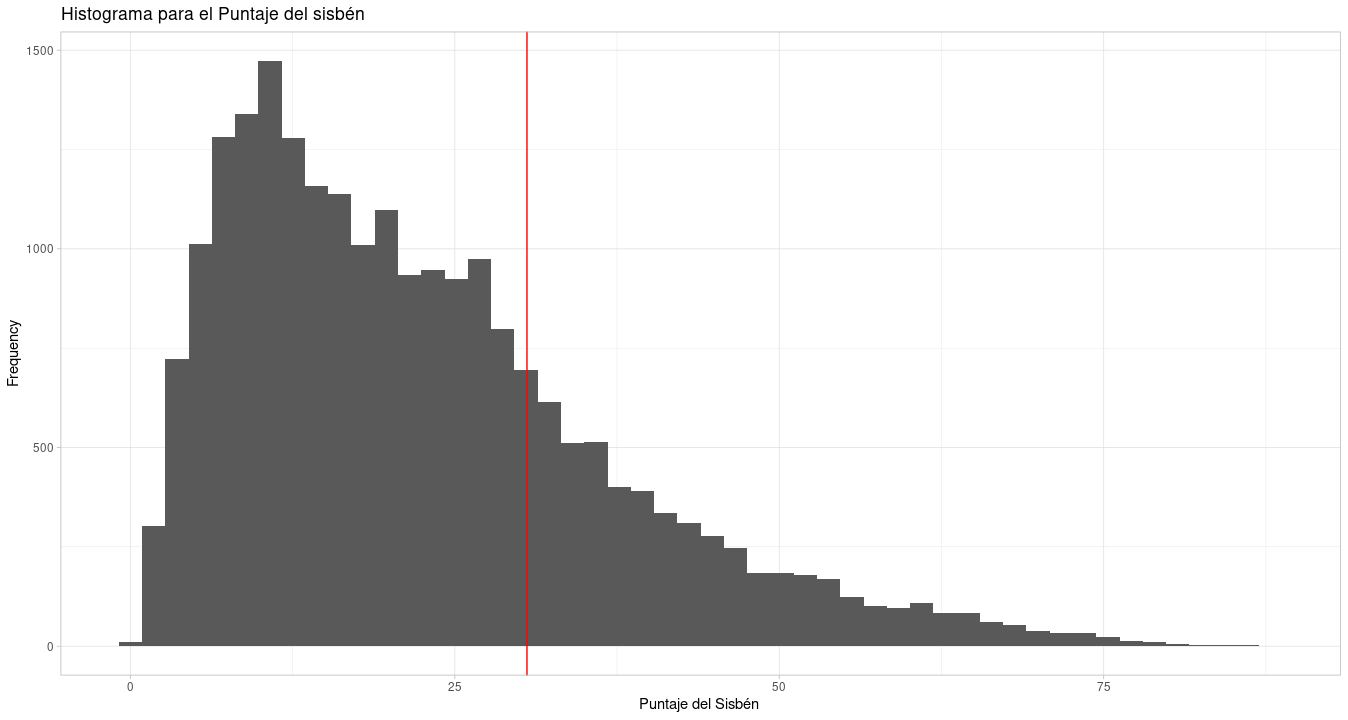
\includegraphics[scale = 0.35]{imagenes/estimax_principal/histrograma_puntaje_sisben.png}
    \caption{El histograma claramente muestra que no hay manipulación por parte de los individuos alrededor del umbral $30.56$ dado la continuidad de la variable puntaje del sisbén 3 alrededor de dicho umbral. La línea vertical roja denota el puntaje de asignación a familias en acción vía puntaje del sisbén.}
    \label{fig:histog_completa}
\end{figure}

Frente a la evidencia estadística de no manipulación, se observa de la figura \ref{fig:histog_completa} que la variable puntaje del sisbén es continua alrededor del umbral por lo que no hay manipulación por parte de los individuos alrededor del umbral.

Esto se complementa con el \textit{test de McCrary} en donde se obtuvo un p-valor de 0.5232 por lo que claramente no se rechaza la hipótesis nula de no manipulación. Lo anterior, se corrobora gráficamente por la continuidad de la gráfica asociada al test de McCrary dada por la figura \ref{fig:mccrary_complete}. 

\begin{figure}[h!]
    \centering
    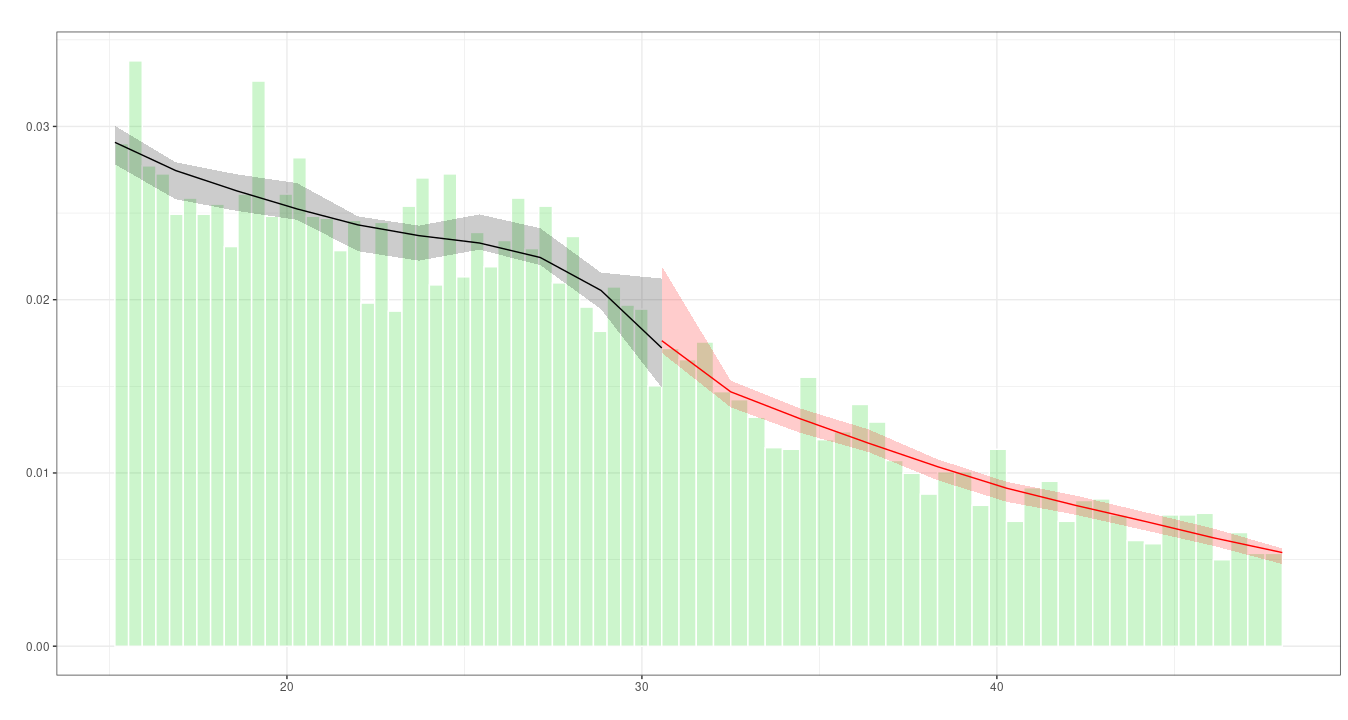
\includegraphics[scale = 0.35]{imagenes/estimax_principal/mccrary_principal.png}
    \caption{Gráfica asociada al Test de McCrary para la estimación principal}
    \label{fig:mccrary_complete}
\end{figure}

\begin{table}[h!]
\centering
\begin{tabular}{lccc}
\hline
\hline
\multicolumn{1}{c}{}    & \multicolumn{3}{c}{Covariadas}                                                                                                                                                     \\ \cline{2-4} 
Características         & \begin{tabular}[c]{@{}c@{}}Sexo\\ (1)\end{tabular}      & \begin{tabular}[c]{@{}c@{}}Embarazada\\ (2)\end{tabular} & \begin{tabular}[c]{@{}c@{}}Percibe Ingreso\\ (3)\end{tabular} \\ \hline
Impacto                 & \begin{tabular}[c]{@{}c@{}}0.045\\ (0.701)\end{tabular} & \begin{tabular}[c]{@{}c@{}}-0.027\\ (0.432)\end{tabular} & \begin{tabular}[c]{@{}c@{}}-0.053\\ (0.871)\end{tabular}      \\
Media                   & 0.52                                                    & 0.025                                                    & 0.07                                                          \\
Controles               & No                                                      & No                                                       & No                                                            \\
Número de observaciones & 22286                                                   & 22286                                                    & 22286    \\ \hline                                                    
\end{tabular}
\caption{Esta tabla contiene las regresiones lineales locales discontinuas usando cada una de las covaridas como variables dependientes en función del puntaje del sisbén. Como se observa, en el umbral $30.56$ el efecto del salto no es significativo. En paréntisis se encuentran los valores de los p-valores.}
\label{tab:cov_main}
\end{table}

Frente a la continuidad de las covariadas, las gráficas \ref{fig:sexo}, \ref{fig:embarazada} y \ref{fig:percibe_ingreso} muestran evidencia gráfica de la continuidad de dichas variables alrededor del umbral. De igual forma, al aplicar un \textit{diseño de regresión lineal local discontinuo} usando cada covariada como variable dependiente y usando el puntaje del sisbén como running variable, basando la estimación en un diseño con kernel rectangular y con un ancho de banda igual a 1, se obtiene los resultados que se presentan en la tabla \ref{tab:cov_main}. Como se puede observar, no hay evidencia estadística de salto alrededor del umbral\footnote{Esto se concluye de la no significancia del impacto}. 

\begin{figure}[h!]
    \centering
    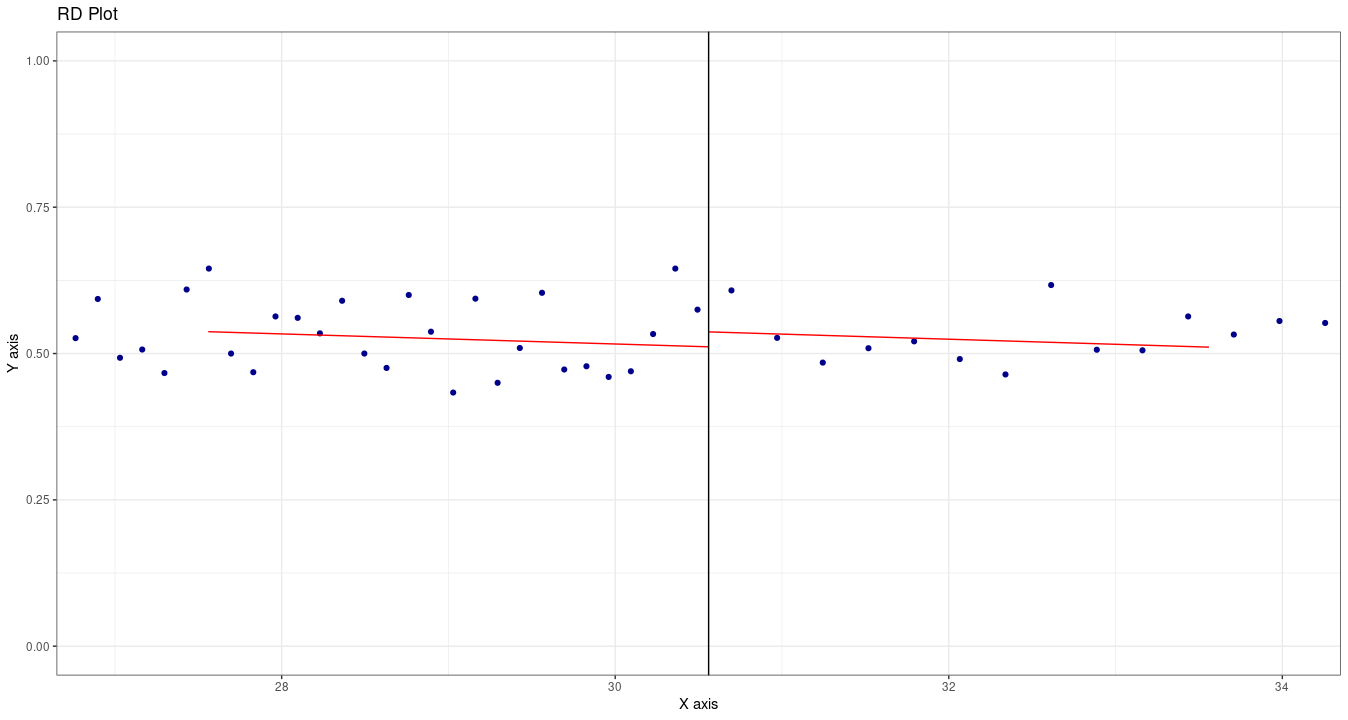
\includegraphics[scale = 0.35]{imagenes/estimax_principal/sexo_main.png}
    \caption{Continuidad de la \textit{covariada sexo} alrededor del umbral}
    \label{fig:sexo}
\end{figure}

\begin{figure}[h!]
    \centering
    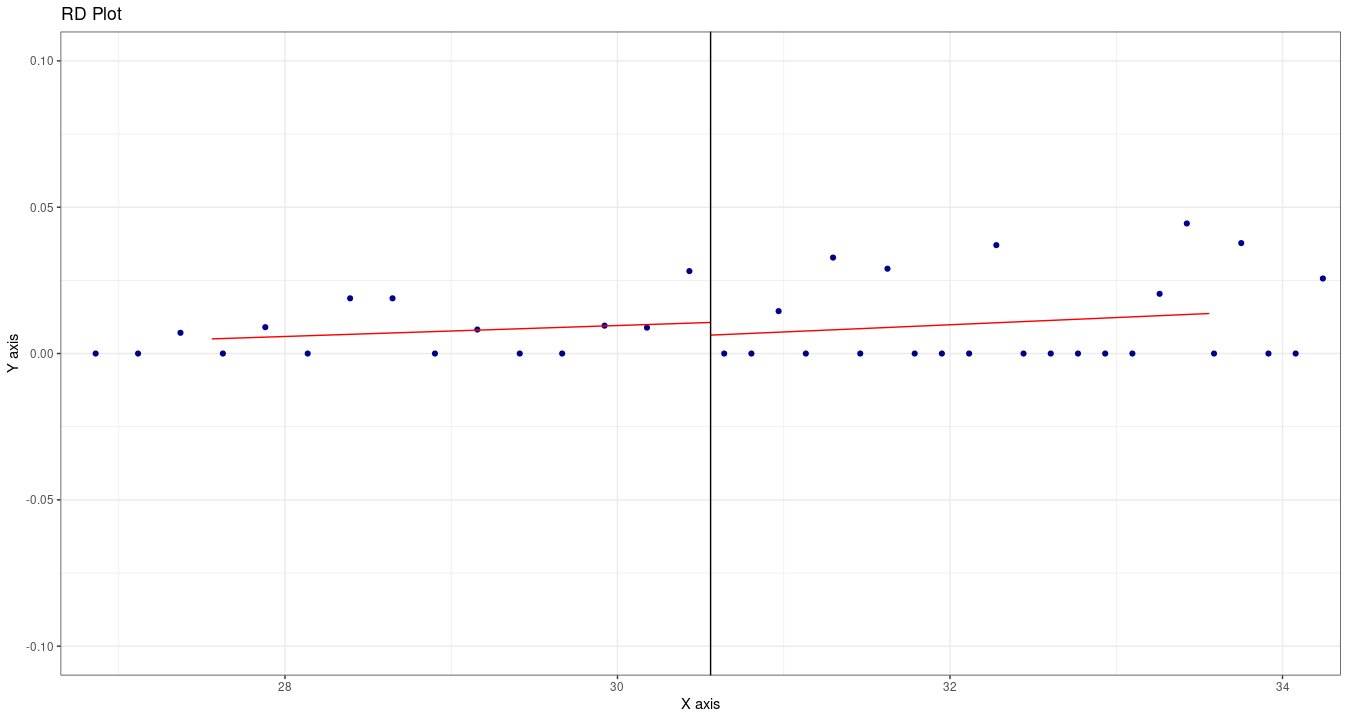
\includegraphics[scale = 0.35]{imagenes/estimax_principal/embarzada_main.png}
    \caption{Continuidad de la \textit{covariada embarazada} alrededor del umbral}
    \label{fig:embarazada}
\end{figure}

\begin{figure}[h!]
    \centering
    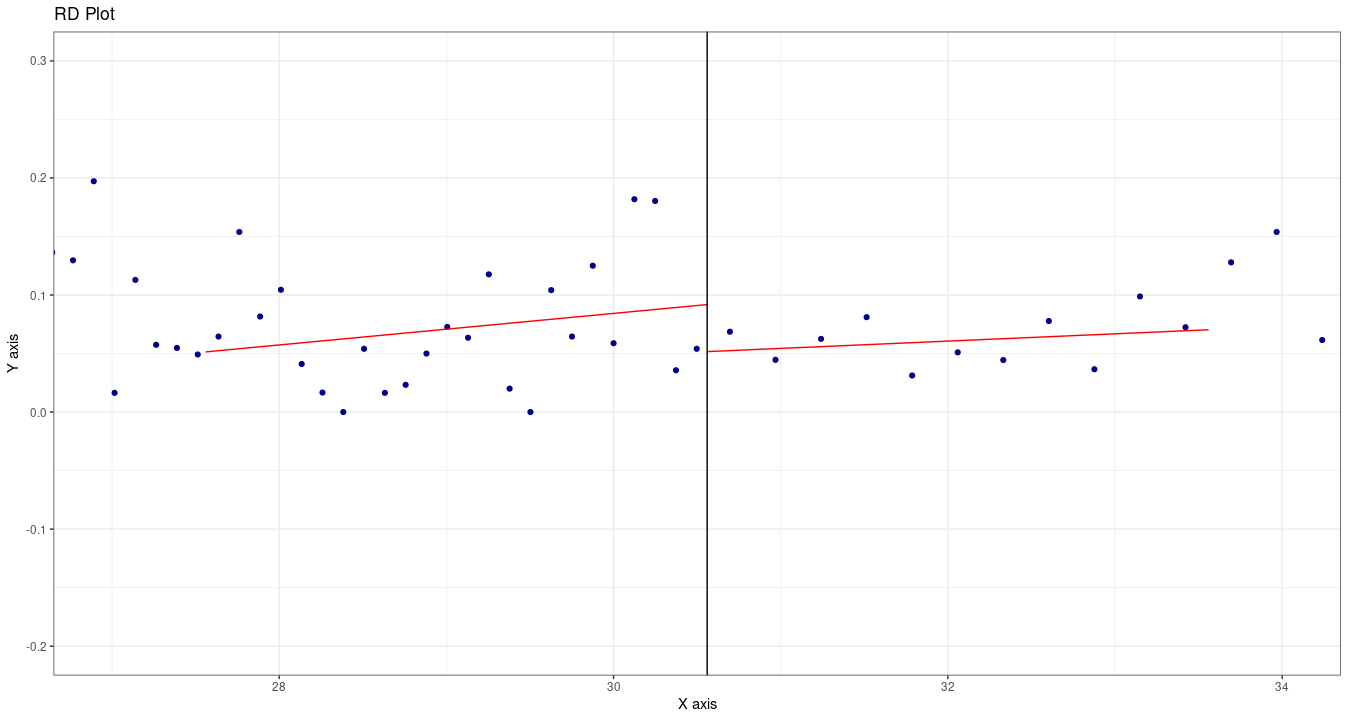
\includegraphics[scale = 0.35]{imagenes/estimax_principal/percibe_ingreso_main.png}
    \caption{Continuidad de la \textit{covariada percibe ingreso} alrededor del umbral}
    \label{fig:percibe_ingreso}
\end{figure}

Por los resultados anteriores, se observa que los dos supuestos de identificación por medio de un RDD se satisfacen\footnote{Estrictamente hablando, no hay evidencia que muestre que haya incumplimiento de los supuestos de identificación dado que en un diseño de investigación de evaluación de impacto no es posible garantizar el total cumplimiento de los supuestos sino la plausibilidad de que dichos supuestos sean ciertos con los datos que se tienen.} por lo que se procede a realizar la estimación principal.

Realizando un \textit{diseño de regresión lineal local discontinuo} con \textit{kernel uniforme} y \textit{ancho de banda} igual a 1 se estima la ecuación asociada a la forma reducida \ref{eq:reduced_form}. Los resultados se presentan en la tabla \ref{tab:estimaxs_principales} y el resultado gráfico del impacto se puede observar en la figura \ref{fig:main_estimax_interes}. 

\begin{table}[h!]
\centering
\begin{tabular}{lcc}
\hline
\hline
\multicolumn{1}{c}{}    & \multicolumn{2}{c}{Estimaciones con toda la muestra}                                                                                     \\ \cline{2-3} 
Características         & \begin{tabular}[c]{@{}c@{}}Estudio el útimo mes\\ (1)\end{tabular} & \begin{tabular}[c]{@{}c@{}}Estudio el último mes\\ (2)\end{tabular} \\ \hline
Impacto                 & \begin{tabular}[c]{@{}c@{}}-0.03**\\ (0.042)\end{tabular}            & \begin{tabular}[c]{@{}c@{}}-0.039**\\ (0.032)\end{tabular}            \\
Media                   & 0.78                                                               & 0.78                                                                \\
Controles               & No                                                                 & Sí                                                                  \\
Número de observaciones & 22286                                                              & 22286   \\ \hline                                                           
\end{tabular}
\caption{Esta tabla contiene las regresiones lineales locales discontinuas usando la variable $EUM$ como variable dependiente en función del puntaje del sisbén. Como se observa, en el umbral $30.56$ el efecto del salto es significativo, por lo que existe una discontinuidad alrededor del umbral causada por encontrarse por encima o debajo del umbral. Para la estimación con controlos, los controles empleados fueron las covariadas: \textit{sexo}, \textit{embarazada} y \textit{percibe ingresos}.En paréntesis se encuentran los valores de los p-valores. Adicionalmente, se utilizó un tipo de \textit{bootstrapping} para el cálculo de los errores robustos utilizados en el cálculo de los p-valores.** denota significancia del 5 \%}
\label{tab:estimaxs_principales}
\end{table}

\begin{figure}[h!]
    \centering
    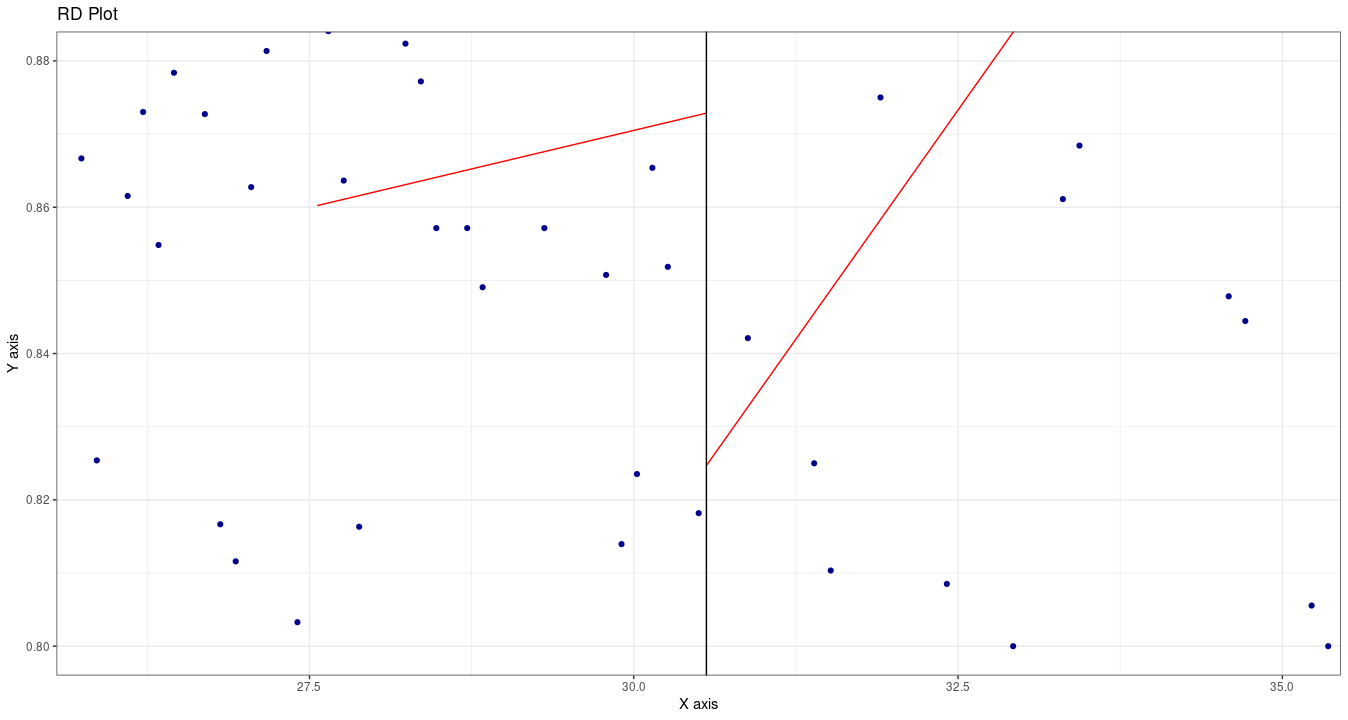
\includegraphics[scale = 0.35]{imagenes/estimax_principal/main_estimax_interes.png}
    \caption{Discontinuidad de la \textit{variable Estudio el último mes (EUM)} alrededor del umbral. El salto representa le estimación del impacto.}
    \label{fig:main_estimax_interes}
\end{figure}

% Intepretación de los resultados

De la tabla \ref{tab:estimaxs_principales} se concluye que la regla institucional de asignación por puntaje de Sisbén a Familias en Acción en el umbral de $30.56$ puntos si tiene un efecto en el acceso a un centro educativo por parte de los niños y jóvenes entre los 6 a 17 años en donde las persona que se encuentran al lado izquierdo del umbral, y por ende pueden ser posibles beneficiarios del programa vía puntaje del Sisbén, tienen una mayor asistencia a un centro educativo que los que se encuentran al lado derecho del umbral como lo muestran los resultados de las estimaciones de la ecuación \ref{eq:reduced_form}. El impacto estimado correspondiente a \ref{eq:impacto} fue de una disminución 3 \% en el acceso a la educación cuando las personas pasan de un nivel un poco más abajo al umbral institucional $30.56$ a estar un poco más arriba del umbral en su puntaje del Sisbén cuando la regresión se hizo sin covariadas y del 4 \% cuando la regresión se hizo con covariadas. Ahora, si se miran dichos impactos respecto a la media de la variable $EUM$, se encuentra un efecto relativo de 4 \% y de 5 \%  sin y con covariadas respectivamente. Estos resultados corroboran que, usando como instrumento el umbral del puntaje del Sisbén en $30.56$ familias en acción si tiene un impacto sobre el acceso a la educación por parte de los niños y jóvenes beneficiados, uno de los principales objetivos de la política. 

% Mencionar lo de inferencia randomizada y placebo
Finalmente, cómo análisis de robustes se decidió realizar inferencia randomizada para calcular el p-valor asociado a la regresión principal, es decir, el p-valor asociado al impacto que tiene el instrumento o la condición de estar por debajo del umbral\footnote{Recordar que el valor de dicho umbral es $30.56$} del puntaje del Sisbén para poder acceder a Familias en Acción sobre el acceso a la educación. Adicionalmente, se decidió realizar dos experimentos placebos en dónde se utilizaban valores de corte o umbral arbitrarios, uno arriba y otro debajo del umbral institucional, con la finalidad de ver si la metodología empleada era robusta a cambios de umbral. Los resultados de lo anterior, se encuentran en el anexo. 

\subsection{Estimaciones auxiliares}

Para complementar la estimación principal, se decidió desagregar las observaciones en los dos grupos poblaciones principales, es decir, un un grupo \textit{g1} que consistía principalmente en niños entre los 6 y 11 años y en un grupo \textit{g2} que consistía principalmente en adolescentes entre los 12 y 17 años y se realizaron las estimaciones con cada grupo. La idea de lo anterior, era ver si existía un efecto diferenciado del umbral institucional sobre el acceso a la educación entre los dos grupos poblacionales mencionados. Los resultados que validan los supuestos para el uso del RDD se encuentran en el anexo. 

Los resultados para una \textit{diseño de regresión lineal local discontinuo} con \textit{kernel uniforme} y \textit{ancho de banda} igual a 1 para estimar la ecuación asociada a la forma reducida \ref{eq:reduced_form} para cada uno de los grupos poblaciones mencionados se encuentran en la tabla \ref{tab:reg_main_grupos} y la evidencia visual de la discontinuidad y no discontinuidad alrededor del umbral en el accesos a la educación para el grupo g1 y para el grupo g2 en las gráficas \ref{fig:estimax_main_g1} y \ref{fig:estimax_main_g2} respectivamente.

\begin{table}[h!]
\begin{tabular}{lcccc}
\hline
\hline
\multicolumn{1}{c}{}    & \multicolumn{2}{c}{\begin{tabular}[c]{@{}c@{}}Estimaciones para el grupo de \\ niños entre 6 a 11 años\end{tabular}}                          & \multicolumn{2}{c}{\begin{tabular}[c]{@{}c@{}}Estimaciones para el grupo de \\ adolescentes entre 12 a 17 años\end{tabular}}                  \\ \cline{2-5} 
Características         & \begin{tabular}[c]{@{}c@{}}Estudio el \\ último mes\\ (1)\end{tabular} & \begin{tabular}[c]{@{}c@{}}Estudio el \\ último mes\\ (2)\end{tabular} & \begin{tabular}[c]{@{}c@{}}Estudio el \\ último mes\\ (3)\end{tabular} & \begin{tabular}[c]{@{}c@{}}Estudio el \\ último mes\\ (4)\end{tabular} \\ \hline
Impacto                 & \begin{tabular}[c]{@{}c@{}}-0.058*\\ (0.098)\end{tabular}             & \begin{tabular}[c]{@{}c@{}}-0.059*\\ (0.092)\end{tabular}             & \begin{tabular}[c]{@{}c@{}}0.007\\ (0.189)\end{tabular}               & \begin{tabular}[c]{@{}c@{}}0.000\\ (0.182)\end{tabular}               \\
Media                   & 0.81                                                                  & 0.81                                                                  & 0.73                                                                  & 0.73                                                                  \\
Controles               & No                                                                    & Sí                                                                    & No                                                                    & Sí                                                                    \\
Número de observaciones & 11683                                                                 & 11683                                                                 & 10603                                                                 & 10603                                                                 \\ \hline
\end{tabular}
\caption{Esta tabla contiene las regresiones lineales locales discontinuas usando la variable $EUM$ como variable dependiente en función del puntaje del sisbén para los grupos g1 y g2. Como se observa, en el umbral $30.56$ el efecto del salto es significativo para el grupo 1, por lo que existe una discontinuidad alrededor del umbral causada por encontrarse por encima o debajo del umbral. No obstante, se encontró que de manera desagregada no hay impacto significativo para el grupo 2. Para las estimaciones con controlos, los controles empleados fueron las covariadas: \textit{sexo}, \textit{embarazada} y \textit{percibe ingresos}. En paréntesis se encuentran los valores de los p-valores. Adicionalmente, se utilizó un tipo de \textit{bootstrapping} para el cálculo de los errores robustos utilizados en el cálculo de los p-valores.* denota significancia del 10 \%}
\label{tab:reg_main_grupos}
\end{table}

\begin{figure}[h!]
    \centering
    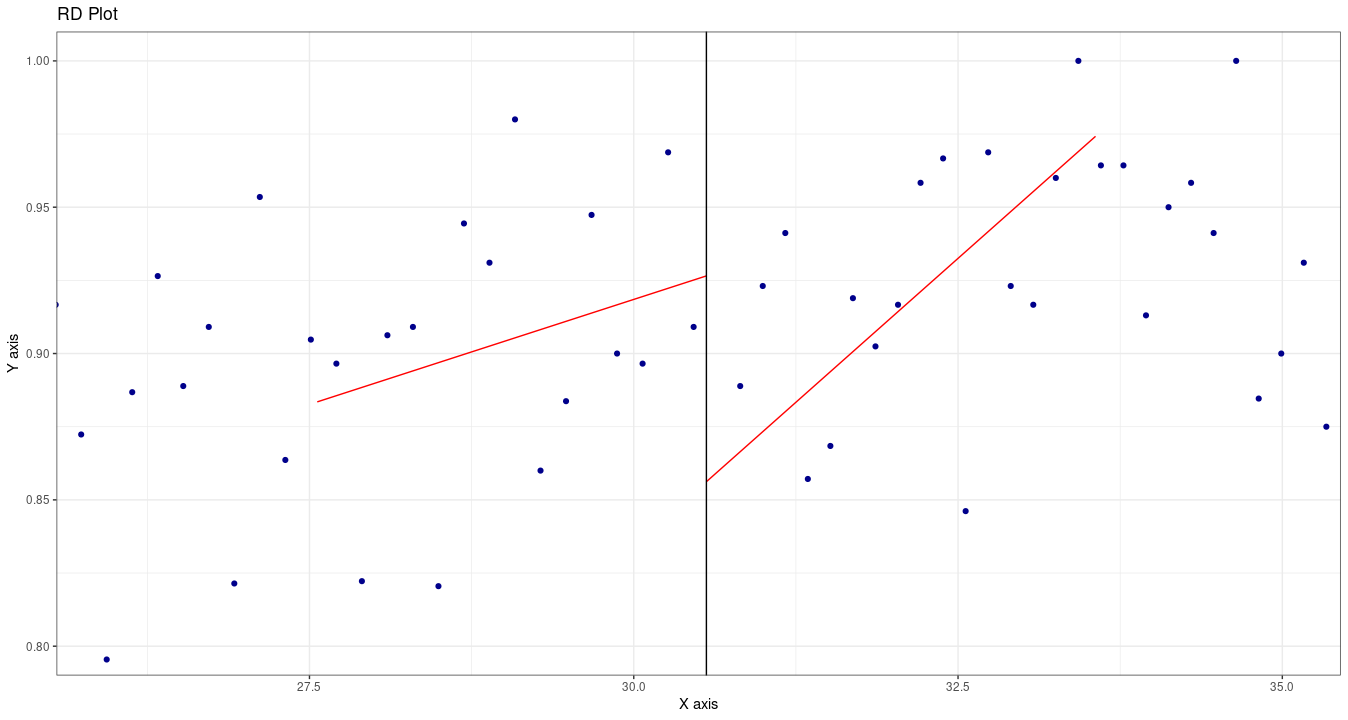
\includegraphics[scale = 0.35]{imagenes/estimaxs_adicionales/g1_estimax.png}
    \caption{Discontinuidad de la \textit{variable Estudio el último mes (EUM)} alrededor del umbral para la estimación con solo el grupo g1. El salto representa le estimación del impacto.}
    \label{fig:estimax_main_g1}
\end{figure}

\begin{figure}[h!]
    \centering
    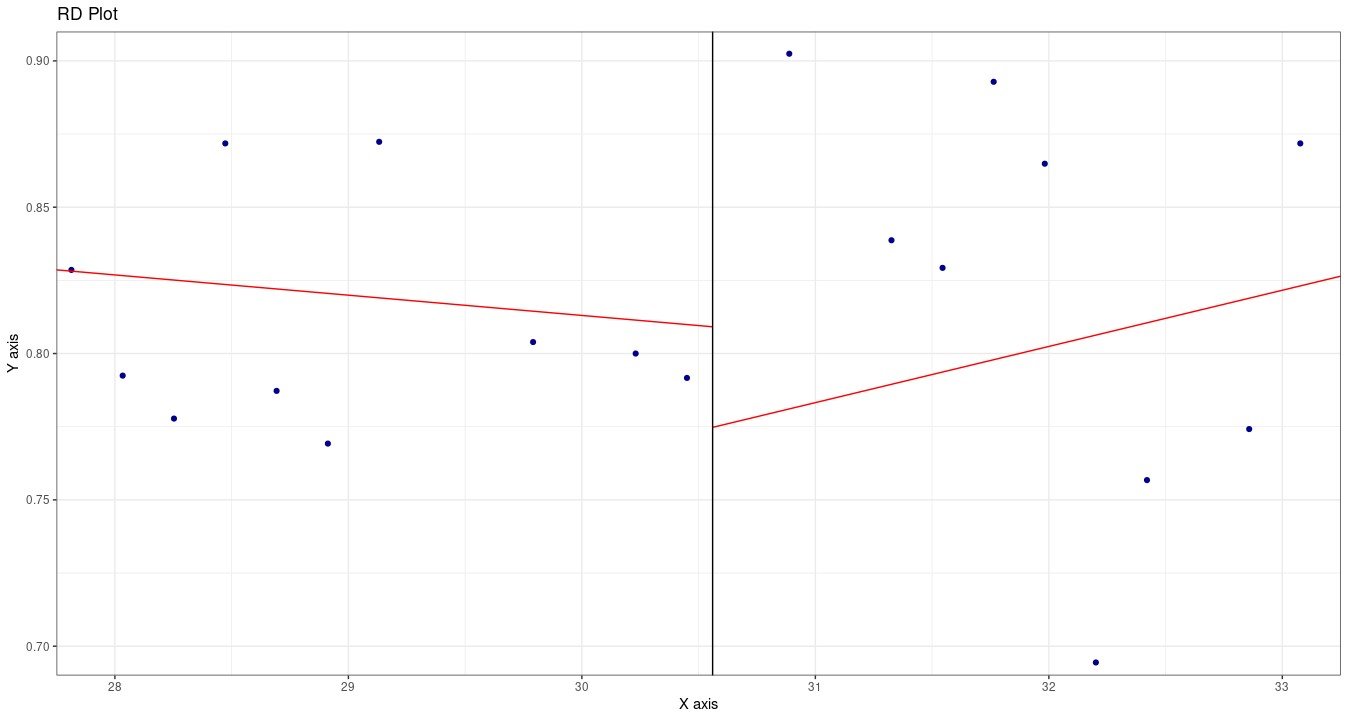
\includegraphics[scale = 0.35]{imagenes/estimaxs_adicionales/g2_estimax.png}
    \caption{Continuidad de la \textit{variable Estudio el último mes (EUM)} alrededor del umbral para la estimación con solo el grupo g2. Por tanto, para este grupo desagregado no hay impacto significativo del umbral institucional en el acceso a la educación.}
    \label{fig:estimax_main_g2}
\end{figure}

% Interprtaciones de los resultados 

De la tabla \ref{tab:estimaxs_principales} se concluye que la regla institucional de asignación por puntaje de Sisbén a Familias en Acción en el umbral de $30.56$ puntos si tiene un efecto en el acceso a un centro educativo por parte de los niños con edades entre 6 a 12 años en donde las persona que se encuentran al lado izquierdo del umbral, y por ende pueden ser posibles beneficiarios del programa vía puntaje del Sisbén, tienen una mayor asistencia a un centro educativo que los que se encuentran al lado derecho del umbral como lo muestran los resultados de las estimaciones de la ecuación \ref{eq:reduced_form}. El impacto estimado correspondiente a \ref{eq:impacto} fue de una disminución del 6 \% en el acceso a la educación cuando las personas pasan de un nivel un poco más abajo al umbral institucional $30.56$ a estar un poco más arriba del umbral en su puntaje del Sisbén cuando la regresión se hizo sin covariadas y también del 6 \% cuando la regresión se hizo con covariadas. Ahora, si se miran dichos impactos respecto a la media de la variable $EUM$, se encuentra un efecto relativo de 7 \%   sin y con covariadas respectivamente. Estos resultados corroboran que, usando como instrumento el umbral del puntaje del Sisbén en $30.56$ familias en acción si tiene un impacto sobre el acceso a la educación por parte de los niños y jóvenes beneficiados en la primera infancia, uno de los principales objetivos de la política. 

Lo interesante, fueron los resultados obtenidos respecto al grupo 2 que cuenta con los adolescentes con edades entre 12 a 17 años. Como lo muestran tanto la tabla \ref{tab:reg_main_grupos} y la gráfica \ref{fig:estimax_main_g2} no existe o al menos no fue posible identificar un efecto significativo del umbral institucional sobre el acceso a la educación por parte de los miembros de éste subgrupo. Existen múltiples razones que explican porque no fue posible encontrar un efecto significativo del umbral en el acceso a la educación por parte de los jóvenes en este rango de edad. La principal razón, a juicio de los autores, consiste en que los individuos alrededor del umbral tiene características en términos socio-económicas y de ingreso muy parecidas por lo que a edades mayores a los 12 años el subsidiado otorgado por familias en acción puede no ser ya un incentivo monetario lo suficientemente fuerte para seguir yendo al colegio. Pero existes otras posibles justificaciones a la no significancia del efecto en este grupo, entre otras, a que a mayor edad existe mayor presión sobre los adolescentes a dejar de estudiar y a conseguir un empleo para ayudar en los ingresos de la familia o simplemente porque los adolescentes sienten que a corto plazo es más provechoso ingreso al mercado laboral, ya sea formal o informal, y conseguir ingresos en lugar de seguir estudiando. 

% Raul, juliana y german
\section{Conclusiones}

Según los resultados mostrados por la literatura y los estudios empíricos, las \textit{transferencias monetarias condicionadas} han sido en general programas efectivos a la hora de aliviar la pobreza de un significativo número de hogares y a incentivar el acceso a la educación y el cuidado de salud de comunidades e individuos marginados en los diferentes países donde se han aplicado y en particular en los países latinoamericanos. 

Los resultados aquí obtenidos, están en la misma dirección que los hallazgos empíricos mostrados por literatura sobre la efectividad e impacto que tienen las TMC's y que dichos impactos sí son significativos, y sobre todo medibles de manera cuantitativa. En particular, se encuentra que existe un impacto de la regla institucional de asignación a familias en acción a partir del puntaje del Sisbén de $30.56$ sobre la accesibilidad a la educación y en particular se identificó un impacto causal de 5 \% en relación a a la media para los niños y adolescentes entre los 6 y 17 años. Por ende, el estudio muestra que efectivamente los TMC's, al menos la principal en Colombia, si ha sido una política pública que ha ayudado a incentivar el acceso a la educación y por ende la formación de capital humano. 

%% Agregar una sección de como estudios futuros pueden mejorar los estudios encontrados en el presente análisis. Dos formas (Dadas las fuertes limitaciones en los datos): 

No obstante, se invita a futuros investigadores y diseñadores de política pública aplicada que sientan útil los hallazgos encontrados acá que extiendan un poco más los resultados obtenidos. En particular, y dado que el Sisbén no es el único mecanismo de asignación, una forma de extender el trabajó realizado sería estimar con una base de datos que claramente identifique que individuos hacen parte de Familias en Acción y que individuos no lo hacen para así lograr realizar la estimación mediante un diseño de investigación de \textit{fuzzy RDD} completo y no limitarse a los resultados que de el instrumento al estimar solamente la \textit{forma reducida} del fuzzy RDD como se hizó en el presente trabajo. De esta forma, empelando un fuzzy RDD, con la base de datos adecuada, es posible identificar el impacto causal y directo que tiene Familias en Acción en el acceso a la educación. 

De igual forma, de obtenerse un panel más completo, en el sentido de tener más observaciones por año y más años de referencia, en lugar de solamente dos años, se podría obtener estimaciones desagregados del impacto del programa en las diferentes regiones del país. En el presente trabajo ello fue imposible dado que no se contaba con la cantidad de datos suficiente por regiones para poder realizar estimaciones con alto poder estadístico. Otra dificultad que se obtuvo acá, fue que no se pudo aislar el efecto de los centros urbanos, dónde se espera que el programa sea menos efectivo, por la misma razón que al filtrar la base de datos para eliminar esas observaciones se pierde mucho poder estadístico en las estimaciones.

% mencionar que no solo es necesario subsidiar la demanda sino también es necesario subsidiar la oferta

% sugerir otros mecanismos de focalización alternativos al sisbén para obtener impactos más significativos

Finalmente, hay cosas que quedan aún por hacer para mejorar la efectividad del programa. En primer lugar, y como lo sugiere \cite{Robles2018Las2001-2018}, es necesario no solo subsidiar la demanda sino también es necesario subsidiar la oferta de tal forma que no solo basta dar subsidios para que las personas puedan estudiar sino también es importante ofrecer más centros educativos y mejorar las instalaciones de los que actualmente existen,de esta forma se podría observar efectos mayores a los que se identificaron en el presente trabajo. De igual forma, otra forma de mejorar la efectividad de familias en acción es mediante la implementación de mecanismos de focalización alternativos al sisen para poder identificar familias que puedan beneficiarse aún más del programa y obtener impactos causales en el acceso a la educación mayores a los obtenidos en el presente artículo.

\clearpage

% german
\section{Anexos}

\subsection{Inferencia randomizada y expermiento placebo para la regresión principal}

\subsubsection{Inferencia randomizada}

Para verificar que en realidad si se encontró un impacto causal significativo se decidió realizar inferencia randomizada para el p-valor del impacto causal estimado en la regresión principal dado por la ecuación \ref{eq:reduced_form}\footnote{En la práctica es muy usual utilizar inferencia randomizada para calcular los errores estándar de los estimadores utilizados en la identificación del impacto y mediante los errores estándar obtenidos mediante dicho procedimiento calcular los respectivos p-valores \citep{Duflo2017HandbookExperiments}}. Se obtuvo un p-valor muy cercano a cero mediante el procedimiento de inferencia randomizada lo que corrobora el resultado obtenido en la regresión principal de la existencia de un impacto significativo de la asignación a familias en acción mediante el umbral del puntaje el sisbén $30.56$ en el acceso a la eduación. 

\subsubsection{Expermientos placebo}

Otro análisis de robustes, ahora para evaluar la calidad de la metodología empleada, fue recrear dicha metodología para la identificación del impacto causal de la regresión principal \ref{eq:reduced_form} pero utilizando umbrales de puntaje del Sisbén arbitarios de tal forma de saber si los resultados también eran o no eran significativos en estos umbrales placebo. 

En el primer experimento placebo, se escoge un umbral de puntaje de sisbén igual a $15$ y se realiza un \textit{diseño de regresión lineal local discontinuo} para la ecuación \ref{eq:reduced_form} usando un kernel uniformo y un ancho de banda igual a 1 mientras que en el segundo experimento placebo se escoge un umbral de puntaje de sisbén igual a $45$ utilizando la misma metodología\footnote{Ambas estimaciones se realizan sin covariadas adicionales}.

\begin{table}[h!]
\begin{tabular}{lcc}
\hline
\hline
\multicolumn{1}{c}{}    & \multicolumn{2}{c}{Estimaciones con toda la muestra}                                                                                                                        \\ \cline{2-3} 
Características         & \begin{tabular}[c]{@{}c@{}}Estudio el útimo mes\\ (umbral placebo = 15)\end{tabular} & \begin{tabular}[c]{@{}c@{}}Estudio el útimo mes\\ (umbral placebo = 45)\end{tabular} \\ \hline
Impacto                 & \begin{tabular}[c]{@{}c@{}}-0.064\\ (0.529)\end{tabular}                             & \begin{tabular}[c]{@{}c@{}}0.028\\ (0.762)\end{tabular}                              \\
Media                   & 0.78                                                                                 & 0.78                                                                                 \\
Controles               & No                                                                                   & Sí                                                                                   \\
Número de observaciones & 22286                                                                                & 22286                                                                                \\ \hline
\end{tabular}
\caption{Esta tabla contiene las regresiones lineales locales discontinuas usando la variable $EUM$ como variable dependiente en función del puntaje del sisbén. Como se observa, en los umbrales placebo $15$ y $45$ el efecto del salto no es significativo, por lo que no existe una discontinuidad alrededor del umbral causada por encontrarse por encima o debajo de los umbrales placebo. Lo anterior, da mayor confianza y robustes a los resultados obtenidos mediante la metodología utilizada para encontrar un efecto significativo en el umbral real.En paréntesis se encuentran los valores de los p-valores. Adicionalmente, se utilizó un tipo de \textit{bootstrapping} para el cálculo de los errores robustos utilizados en el cálculo de los p-valores.** denota significancia del 5 \%}
\label{tab:placebo}
\end{table}

Como muestra la tabla de resultados \ref{tab:placebo}, claramente los impactos no son significativos cuándo se introducen umbrales placebos arbitrarios lo que da mayor robustez al procedimiento empleado para la identificación del impacto causal \ref{eq:impacto}. Adicionalmente, las gráficas \ref{fig:placebo1} y \ref{fig:placebo2} muestran que hay continuidad alrededor de los umbrales placebos escogidos arbitrariamente lo que reafirma los resultados de la tabla \ref{tab:placebo}.

\begin{figure}[h!]
    \centering
    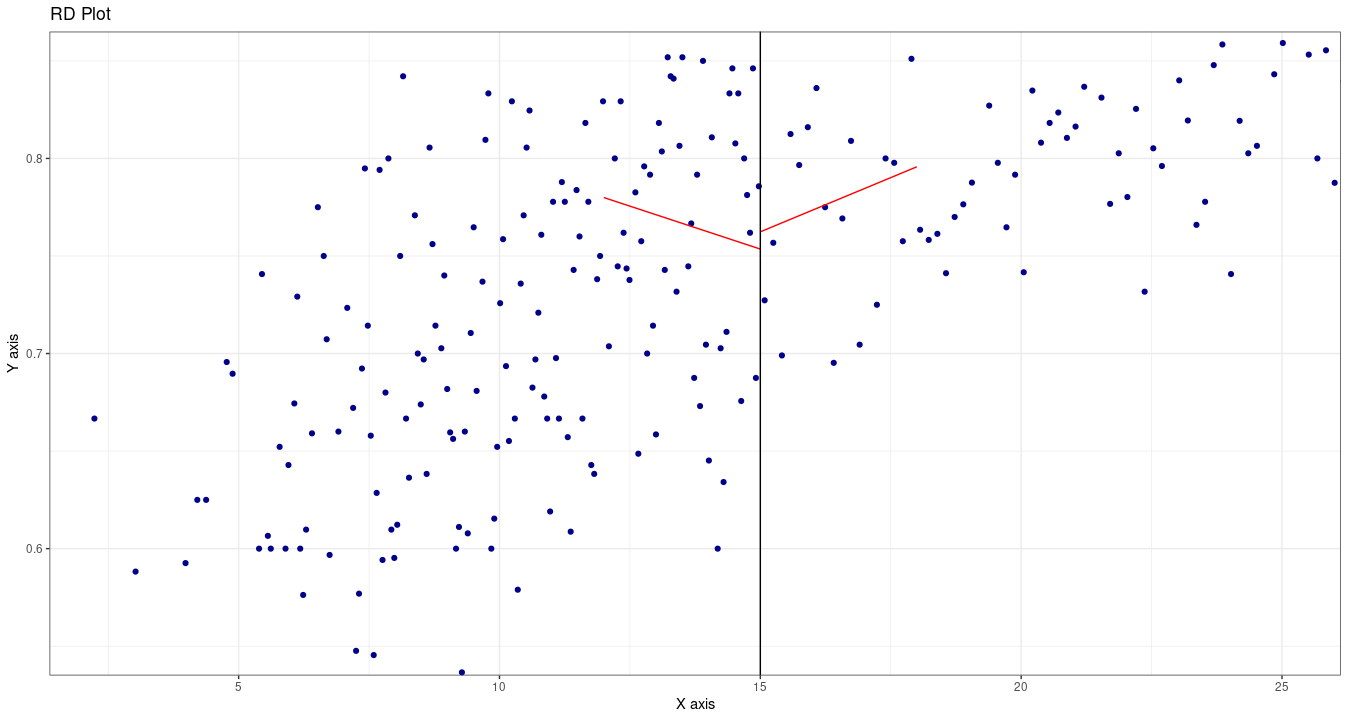
\includegraphics[scale = 0.35]{imagenes/estimax_principal/placebo1_main.png}
    \caption{Continuidad de la \textit{variable Estudio el último mes (EUM)} alrededor del umbral placebo puntaje del Sisbén$15$.}
    \label{fig:placebo1}
\end{figure}

\begin{figure}[h!]
    \centering
    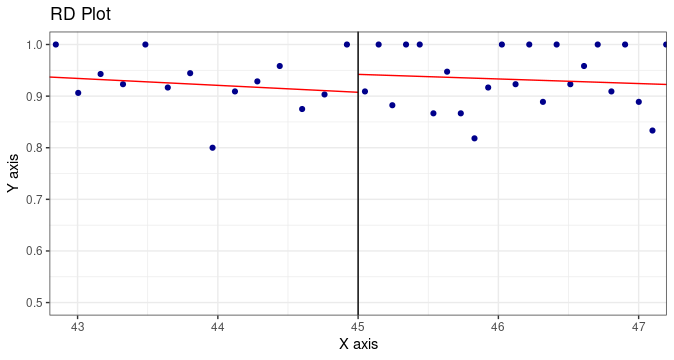
\includegraphics[scale = 0.35]{imagenes/estimax_principal/placebo2_main.png}
    \caption{Continuidad de la \textit{variable Estudio el último mes (EUM)} alrededor del umbral placebo puntaje del Sisbén$45$.}
    \label{fig:placebo2}
\end{figure}

\subsection{Validación de supuestos para las regresiones auxiliares}

A continuación se muestran los resultado que garantizan el cumplimiento de los supuestos de: 1) no manipulación alrededor del umbral y 2) continuidad de las covariada alrededor del umbral, para los grupos poblaciones desagregados: g1) niños entre 6 a 11 años y g2) adolescentes entre 12 a 17 años. 

\subsubsection{Grupo poblacional 1: Niños entre 6 a 11 años}

El grupo poblacional g1 no muestra manipulación alrededor del umbral como lo muestra el resultado de un \textit{test de McCrary} en donde se rechaza la hipótesis nula de no manipulación con p-valor de $0.293$. De igual forma, tanto el histograma \ref{fig:hist_g1} como la visualización gráfica de la prueba McCrary \ref{fig:mccrary_g1} muestran que no hay manipulación por parte de este grupo alrededor del umbral. 

\begin{figure}[h!]
    \centering
    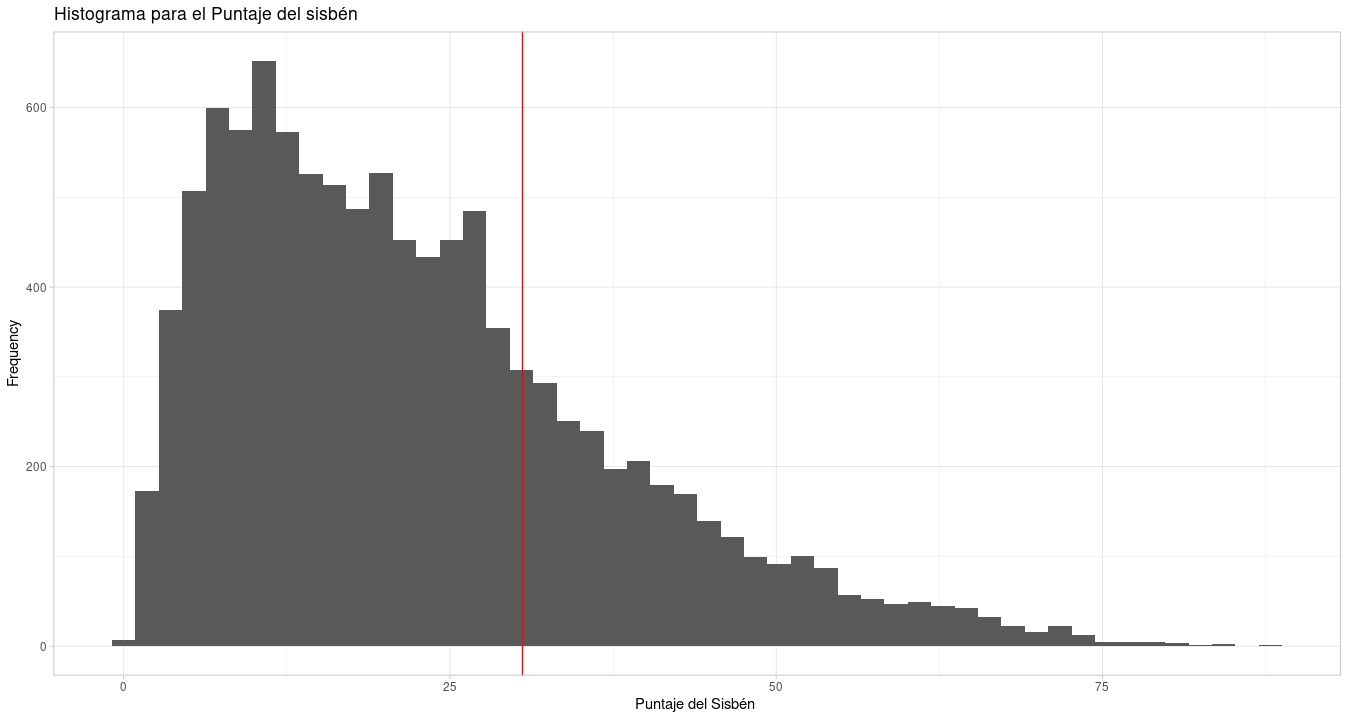
\includegraphics[scale = 0.35]{imagenes/estimaxs_adicionales/histograma_g1.png}
    \caption{El histograma claramente muestra que no hay manipulación por parte del grupo poblacional que conforma g1 alrededor del umbral $30.56$ dado la continuidad de la variable puntaje del sisbén 3 alrededor de dicho umbral. La línea vertical roja denota el puntaje de asignación a familias en acción vía puntaje del sisbén.}
    \label{fig:hist_g1}
\end{figure}

\begin{figure}[h!]
    \centering
    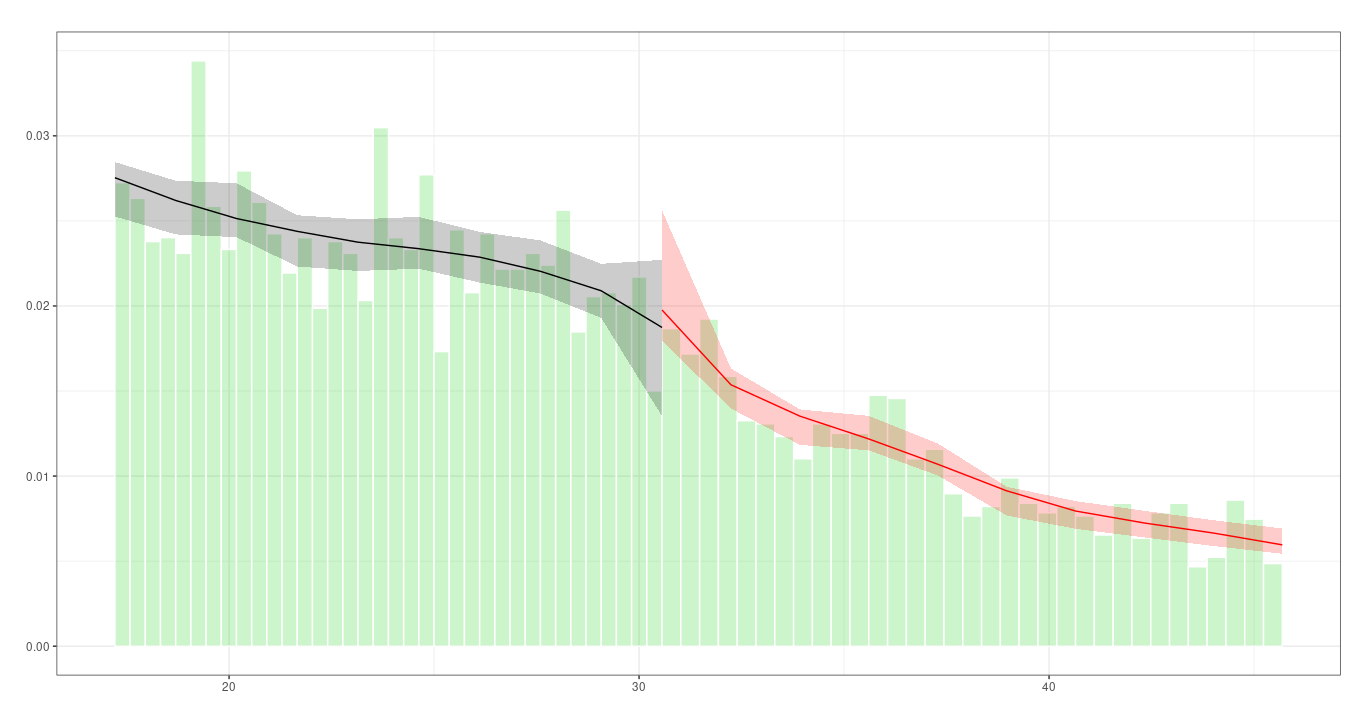
\includegraphics[scale = 0.35]{imagenes/estimaxs_adicionales/mccrary_g1.png}
    \caption{Gráfica asociada al Test de McCrary para la estimación principal con solo el grupo g1}
    \label{fig:mccrary_g1}
\end{figure}

De igual forma, no hay evidencia de discontinuidad en las covariadas \textit{sexo}, \textit{embarazada} y \textit{percibe ingreso} cuando se hacen las estimaciones correspondientes con solo el grupo g1 por lo que concluye que no hay explicaciones plausibles alternativas por parte de las covariadas manejadas sobre el efecto del umbral institucional. Los resultados de esta no significancia se encuentran en la tabla \ref{tab:cov_g1}. 

\begin{table}[h!]
\begin{tabular}{lccc}
\hline
\hline
\multicolumn{1}{c}{}    & \multicolumn{3}{c}{Covariadas}                                                                                                                                                      \\ \cline{2-4} 
Características g1      & \begin{tabular}[c]{@{}c@{}}Sexo\\ (1)\end{tabular}       & \begin{tabular}[c]{@{}c@{}}Embarazada\\ (2)\end{tabular} & \begin{tabular}[c]{@{}c@{}}Percibe Ingreso\\ (3)\end{tabular} \\ \hline
Impacto                 & \begin{tabular}[c]{@{}c@{}}-0.011\\ (0.506)\end{tabular} & \begin{tabular}[c]{@{}c@{}}-0.002\\ (0.320)\end{tabular} & \begin{tabular}[c]{@{}c@{}}-0.078\\ (0.611)\end{tabular}      \\
Media                   & 0.51                                                     & 0                                                        & 0.06                                                          \\
Controles               & No                                                       & No                                                       & No                                                            \\
Número de observaciones & 11683                                                    & 11683                                                    & 11683 \\ \hline                                                        
\end{tabular}
\caption{Esta tabla contiene las regresiones lineales locales discontinuas usando cada una de las covaridas como variables dependientes en función del puntaje del sisbén para el grupo g1. Como se observa, en el umbral $30.56$ el efecto del salto no es significativo. En paréntisis se encuentran los valores de los p-valores.}
\label{tab:cov_g1}
\end{table}

\subsubsection{Grupo poblacional 2: Adolescentes entre 12 a 17 años}

El grupo poblacional g2 no muestra manipulación alrededor del umbral como lo muestra el resultado de un \textit{test de McCrary} en donde se rechaza la hipótesis nula de no manipulación con p-valor de $0.30$. De igual forma, tanto el histograma \ref{fig:hist_g2} como la visualización gráfica de la prueba McCrary \ref{fig:mccrary_g2} muestran que no hay manipulación por parte de este grupo alrededor del umbral. 

\begin{figure}[h!]
    \centering
    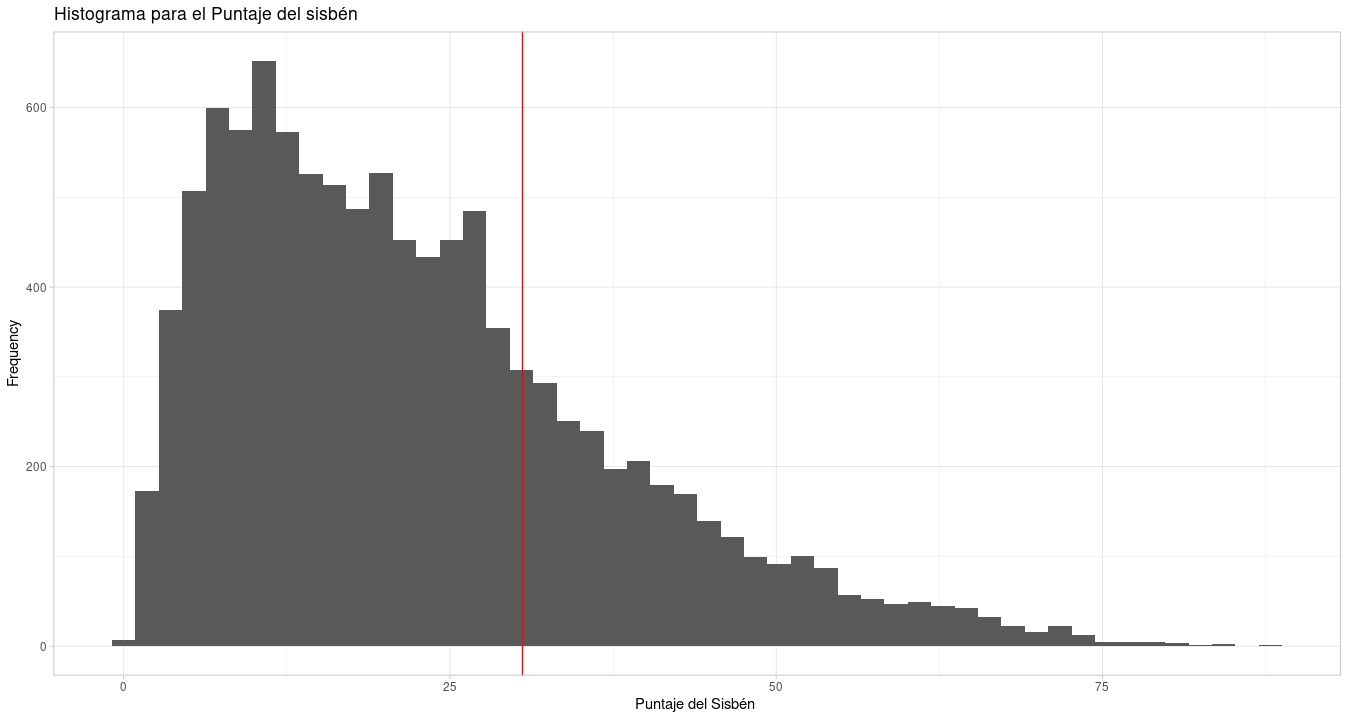
\includegraphics[scale = 0.35]{imagenes/estimaxs_adicionales/histograma_g2.png}
    \caption{El histograma claramente muestra que no hay manipulación por parte del grupo poblacional que conforma g2 alrededor del umbral $30.56$ dado la continuidad de la variable puntaje del sisbén 3 alrededor de dicho umbral. La línea vertical roja denota el puntaje de asignación a familias en acción vía puntaje del sisbén.}
    \label{fig:hist_g2}
\end{figure}

\begin{figure}[h!]
    \centering
    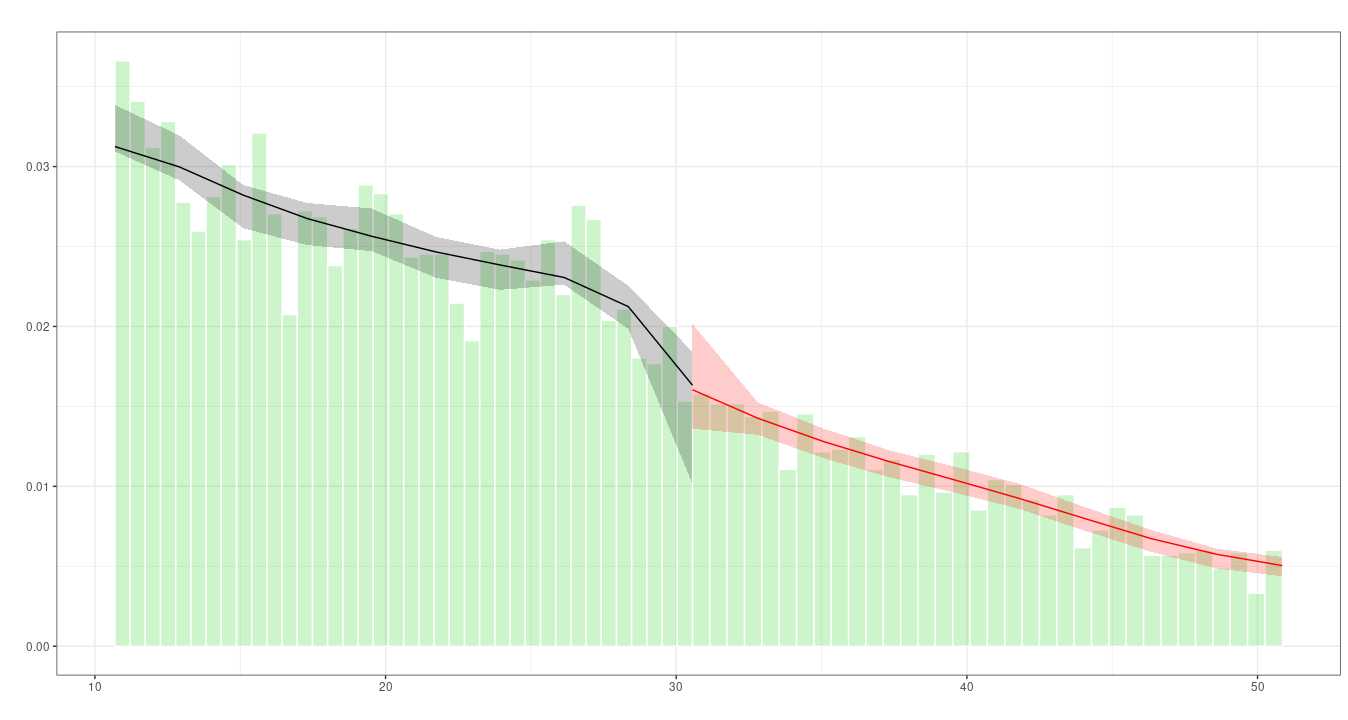
\includegraphics[scale = 0.35]{imagenes/estimaxs_adicionales/mccrary_g2.png}
    \caption{Gráfica asociada al Test de McCrary para la estimación principal con solo el grupo g2}
    \label{fig:mccrary_g2}
\end{figure}

\newpage

De igual forma, no hay evidencia de discontinuidad en las covariadas \textit{sexo}, \textit{embarazada} y \textit{percibe ingreso} cuando se hacen las estimaciones correspondientes con solo el grupo g2 por lo que concluye que no hay explicaciones plausibles alternativas por parte de las covariadas manejadas sobre el efecto del umbral institucional. Los resultados de esta no significancia se encuentran en la tabla \ref{tab:cov_g2}. 

\begin{table}[h!]
\begin{tabular}{lccc}
\hline
\hline
\multicolumn{1}{c}{}    & \multicolumn{3}{c}{Covariadas}                                                                                                                                                      \\ \cline{2-4} 
Características g2      & \begin{tabular}[c]{@{}c@{}}Sexo\\ (1)\end{tabular}       & \begin{tabular}[c]{@{}c@{}}Embarazada\\ (2)\end{tabular} & \begin{tabular}[c]{@{}c@{}}Percibe Ingreso\\ (3)\end{tabular} \\ \hline
Impacto                 & \begin{tabular}[c]{@{}c@{}}0.117 \\ (0.883)\end{tabular} & \begin{tabular}[c]{@{}c@{}}-0.057\\ (0.514)\end{tabular} & \begin{tabular}[c]{@{}c@{}}-0.018\\ (0.244)\end{tabular}      \\
Media                   & 0.52                                                     & 0.052                                                        & 0.082                                                          \\
Controles               & No                                                       & No                                                       & No                                                            \\
Número de observaciones & 10603                                                    & 10603                                                    & 10603 \\ \hline                                                        
\end{tabular}
\caption{Esta tabla contiene las regresiones lineales locales discontinuas usando cada una de las covaridas como variables dependientes en función del puntaje del sisbén para el grupo g2. Como se observa, en el umbral $30.56$ el efecto del salto no es significativo. En paréntisis se encuentran los valores de los p-valores.}
\label{tab:cov_g2}
\end{table}

\clearpage

\bibliography{references.bib}

\end{document}